\documentclass[12pt, a4paper, oneside, openright]{book}

% --- Pacchetti Fondamentali ---
\usepackage[utf8]{inputenc}
\usepackage[T1]{fontenc}
\usepackage[italian]{babel} % Gestione lingua italiana
\usepackage{csquotes}       % Consigliato con babel
\usepackage{graphicx}       % Per le immagini
\usepackage{hyperref}       % Per i link cliccabili e indice
\usepackage{geometry}       % Margini
\geometry{a4paper, top=3cm, bottom=3cm, left=3.5cm, right=2.5cm}
\usepackage{amsmath}
\linespread{1.5}
\usepackage{tcolorbox}
\usepackage{tikz}
\def\checkmark{\tikz\fill[scale=0.4](0,.35) -- (.25,0) -- (1,.7) -- (.25,.15) -- cycle;}
\usepackage{booktabs}

\usepackage[a-1b]{pdfx}

% --- Gestione Bibliografia ---
\usepackage[backend=biber, style=numeric, sorting=none]{biblatex}
\addbibresource{references.bib}

% --- Gestione Codice (Smart Contracts / Python) ---
\usepackage{listings}
\usepackage{xcolor}
\definecolor{codegray}{rgb}{0.5,0.5,0.5}
\definecolor{backcolour}{rgb}{0.95,0.95,0.92}

% ---Grafici ---

\usepackage{pgfplots}
\pgfplotsset{compat=1.18}
\usepackage{subcaption} % Per affiancare i grafici
\usepackage{tikz}
\usetikzlibrary{shapes, arrows, positioning}

% Configurazione stile codice
\lstdefinestyle{mystyle}{
    backgroundcolor=\color{backcolour},   
    commentstyle=\color{green},
    keywordstyle=\color{blue},
    numberstyle=\tiny\color{codegray},
    stringstyle=\color{red},
    basicstyle=\ttfamily\footnotesize,
    breakatwhitespace=false,         
    breaklines=true,                 
    captionpos=b,                    
    keepspaces=true,                 
    numbers=left,                    
    numbersep=5pt,                  
    showspaces=false,                
    showstringspaces=false,
    showtabs=false,                  
    tabsize=2
}
\lstset{style=mystyle}

% --- Inizio Documento ---
\begin{document}

\frontmatter

\begin{titlepage}
    \begin{center}
        
\includegraphics[width=0.2\textwidth]{images/unisa.png} \\
        {{\large \textbf{Università degli Studi di Salerno}}} \\
        \vspace{3mm}
        {\large Dipartimento di Informatica} \\

         \rule{0.5\textwidth}{0.4pt}
        
        {\small Corso di Laurea Magistrale in Informatica}
        
        \vspace{15mm} 
        
        {\large \textbf{Tesi di Laurea Magistrale}} \\
        
        \vspace{20mm}
        
        % Titolo della tesi
        {\LARGE \textbf{LLM-BASED VULNERABILITY DETECTION FOR SMART CONTRACTS: FINE-TUNING AND RAG}}
        
    \end{center}
    
    \vspace{25mm}
    
    \begin{minipage}[t]{0.47\textwidth}
        \textbf{Relatore:} \\
        Prof. Christiancarmine Esposito \\
        
    \end{minipage}
    \hfill
    \begin{minipage}[t]{0.47\textwidth}
        \raggedleft
        \textbf{Candidato:} \\
        Nicola Tortora \\
        Matricola: 0522501445
    \end{minipage}
    
    \vspace{30mm}
    
    \begin{center}
        \rule{0.5\textwidth}{0.4pt} \\ % Linea orizzontale
        \vspace{3mm}
        \textbf{Anno Accademico 2025/2026}
    \end{center}
    
\end{titlepage}

 

\chapter*{Abstract}
% Contesto e Motivazioni
L'ecosistema blockchain di Algorand, pur offrendo elevate prestazioni e sicurezza nativa, sconta attualmente una severa carenza di strumenti automatizzati per l'analisi dei suoi Smart Contract, sviluppati tramite il linguaggio PyTeal. Parallelamente, i recenti Large Language Models (LLM) hanno dimostrato grandi potenzialità nell'analisi del codice, ma se applicati in modalità \textit{zero-shot} alla sicurezza software tendono a degenerare nella ricerca di correlazioni sintattiche superficiali, risultando proni ad allucinazioni e incapaci di dedurre la reale logica causale delle vulnerabilità. 


% Metodologia
Per superare queste limitazioni, questa tesi propone e valuta una pipeline di \textit{Vulnerability Detection} ibrida e \textit{LLM-Centric}, specificamente ottimizzata per l'ecosistema Algorand. Il framework analizza l'impatto di due metodologie avanzate: l'adattamento al dominio tramite \textbf{Fine-Tuning supervisionato basato su esempi Chain-of-Thought (CoT)} --- mirato a istruire il modello a generare un ragionamento analitico passo-passo --- e l'integrazione di contesto dinamico tramite \textbf{Retrieval-Augmented Generation (RAG)}. Per ovviare ai bias semantici del recupero basato su codice grezzo, il modulo RAG implementato sfrutta un'\textbf{astrazione semantica} ad alto livello del codice. Questa astrazione abilita un \textit{In-Context Learning} mirato: recuperando esempi di codice vulnerabile pertinenti e descrizioni di sicurezza per iniettarli direttamente nel \textit{prompt}, il sistema fornisce all'LLM riferimenti logici chiari per guidarne l'analisi.

% Risultati
I risultati sperimentali dimostrano l'efficacia dell'approccio proposto, evidenziando in particolare il netto incremento prestazionale apportato dalle metodologie rispetto agli approcci tradizionali. L'integrazione del RAG si è rivelata di grande impatto: agendo come meccanismo di validazione fattuale e abbattendo drasticamente i falsi positivi, ha garantito un miglioramento sostanziale dell'F1-Score e della Recall rispetto alle \textit{baseline} in \textit{zero-shot}. Questo ha permesso ai modelli di grossa taglia (come DeepSeek V3.2) di rasentare l'accuratezza ideale senza necessità di addestramento specifico. Al contempo, l'addestramento specifico ha ridotto sensibilmente la tendenza alle allucinazioni dei modelli di taglia media (come \texttt{QwQ-32B}), fornendo loro le competenze necessarie per condurre i task di audit in maniera molto più rigorosa e approfondita rispetto alla controparte base.

% Conclusioni
I risultati sperimentali evidenziano come la necessità del Fine-Tuning dipenda fortemente dalla dimensione del modello. Se nei modelli massivi l'\textit{In-Context Learning} tramite RAG è sufficiente per ottenere risultati ottimali,
per i modelli di taglia media l'addestramento specifico rimane determinante per condurre audit rigorosi in ambienti privati (\textit{on-premise}), colmando di fatto il distacco rispetto alle più costose soluzioni commerciali.

Il presente lavoro costituisce uno dei primi framework di sicurezza basati su IA ottimizzati per PyTeal. Al fine di garantire la totale riproducibilità scientifica, l'intero codice sorgente, i dataset generati e le configurazioni dei modelli sono stati resi pubblicamente disponibili con licenza open-source.



\tableofcontents
\listoffigures

\mainmatter

% --- Capitoli ---
\chapter{Introduzione}
\section{Contesto e Motivazione}
La tecnologia Blockchain ha ridefinito il concetto di fiducia digitale e decentralizzazione, permettendo lo scambio di valore e l'esecuzione di logiche complesse senza intermediari. Al centro di questa rivoluzione vi sono gli \textit{Smart Contract}, programmi immutabili che eseguono automaticamente clausole contrattuali al verificarsi di determinate condizioni. Tra le piattaforme di nuova generazione, \textbf{Algorand} si distingue per il suo protocollo di consenso \textit{Pure Proof-of-Stake} (PPoS), che garantisce scalabilità, sicurezza e finalità immediata delle transazioni.

Tuttavia, l'immutabilità della blockchain rappresenta un'arma a doppio taglio: una volta distribuito, il codice di uno smart contract non può essere modificato. Di conseguenza, eventuali vulnerabilità di sicurezza possono portare a perdite economiche ingenti e irreversibili. La sicurezza del codice diventa quindi un requisito non funzionale critico, specialmente in un ecosistema in cui gli asset gestiti hanno un valore monetario reale.

In ambito Algorand, lo sviluppo di smart contract avviene principalmente tramite l'Algorand Virtual Machine (AVM) e linguaggi di alto livello come \textbf{PyTeal} (un binding Python che compila in TEAL - \textit{Transaction Execution Approval Language}). La specificità e la complessità di questo stack tecnologico rendono l'audit di sicurezza particolarmente sfidante.

\section{Definizione del Problema}
Attualmente, la rilevazione di vulnerabilità negli smart contract si affida prevalentemente a due approcci, entrambi con limitazioni significative:

\begin{enumerate}
    \item \textbf{Strumenti di Analisi Statica}: Sebbene efficaci nell'individuare pattern noti e violazioni sintattiche, questi strumenti spesso mancano di "comprensione semantica". Tendono a generare un elevato numero di falsi positivi (segnalando errori dove non ci sono) o, peggio, falsi negativi (mancando vulnerabilità logiche complesse che dipendono dal contesto dell'applicazione).
    
    \item \textbf{Large Language Models (LLM)}: Modelli come GPT-5, Gemini o DeepSeek, dimostrano capacità di ragionamento eccezionali. Tuttavia, la loro performance degrada sensibilmente quando operano su linguaggi di dominio specifico e di nicchia come PyTeal. A differenza di Solidity (Ethereum), che è ampiamente rappresentato nei dataset di addestramento pubblici, PyTeal e TEAL sono meno diffusi. Di conseguenza, gli LLM generalisti tendono a "allucinare" sintassi inesistenti o a non comprendere le sottili implicazioni di sicurezza specifiche dell'AVM (es. gestione del \textit{rekeying} o utilizzo degli opcode).
\end{enumerate}

\section{Obiettivi e Contributo della Tesi}
L'obiettivo di questo lavoro di tesi è colmare il divario tra la potenza di ragionamento degli LLM moderni e la necessità di una conoscenza tecnica specifica per la sicurezza su Algorand. 

Al fine di superare tali limitazioni e ottimizzare le prestazioni degli attuali Large Language Models (LLM), in questo lavoro di tesi si propongono e si valutano due metodologie avanzate:

\begin{itemize}
    \item \textbf{Fine-tuning (Adattamento del Modello)}: Addestramento di un LLM open-source su un dataset curato di smart contract PyTeal e relative vulnerabilità note. Questo processo serve ad adattare il modello al linguaggio target, migliorandone la capacità di comprendere la sintassi e la struttura logica specifica di Algorand.
    
    \item \textbf{Retrieval-Augmented Generation (RAG)}: Integrazione del modello con una base di conoscenza esterna (Knowledge Base) contenente la documentazione aggiornata sulle vulnerabilità di Algorand. Il RAG permette al modello di accedere a informazioni di contesto mirate durante la fase di inferenza, riducendo le allucinazioni e garantendo che l'analisi sia conforme alle specifiche più recenti.
\end{itemize}

\section{Struttura dell'Elaborato}
Il presente documento è organizzato come segue:
\begin{itemize}
    \item Il \textbf{Capitolo 2} fornisce il background necessario sulla blockchain Algorand, il linguaggio PyTeal, le vulnerabilità comuni, una base teoriaca sugli LLM e RAG.
    \item Il \textbf{Capitolo 3} presenta lo stato dell'arte e ne descrive le problematiche e come tentiamo di migliorarle.
    \item Il \textbf{Capitolo 4} descrive la metodologia proposta, inclusa la preparazione del dataset, il processo di fine-tuning e l'implementazione della pipeline RAG.
    \item Il \textbf{Capitolo 5} presenta i risultati sperimentali.
    \item Il \textbf{Capitolo 6} trae le conclusioni e delinea possibili sviluppi futuri.
\end{itemize}

\chapter{Background}
\section{Algorand e l'Ecosistema di Sviluppo Smart Contract}
\label{sec:algorand_background}

Per comprendere la natura delle vulnerabilità analizzate in questa tesi, è necessario delineare le caratteristiche dell'infrastruttura Algorand. A differenza delle blockchain EVM-based, Algorand adotta un paradigma architetturale che separa nettamente il livello del consenso dalla logica applicativa, introducendo primitive di sicurezza uniche che influenzano direttamente le superfici di attacco.

\subsection{L'Architettura AVM e il Modello Transazionale}
Alla base dell'esecuzione degli smart contract vi è la \textit{Algorand Virtual Machine} (AVM), un interprete stack-based non Turing-completo (nella sua concezione originale) progettato per massimizzare la velocità di verifica.
L'AVM opera all'interno di un protocollo di consenso \textit{Pure Proof-of-Stake} (PPoS), che garantisce finalità immediata delle transazioni: una volta che un blocco è scritto, non può essere "forkato". Dal punto di vista della sicurezza del codice, tre caratteristiche dell'AVM sono determinanti:

\begin{itemize}
    \item \textbf{Algorand Standard Assets (ASA):} A differenza di Ethereum, dove i token sono smart contract (ERC-20), su Algorand gli asset sono primitive di primo livello gestite direttamente dal protocollo. Ciò elimina intere classi di vulnerabilità come la \textit{Reentrancy}, ma introduce rischi specifici legati alla gestione dei permessi di trasferimento.
    \item \textbf{Modello di Stato Duale:} Gli smart contract (\textit{Stateful Applications}) possono manipolare due tipi di memoria:
    \begin{itemize}
        \item \textit{Global State:} Variabili associate all'applicazione stessa (es. contatori totali, admin address).
        \item \textit{Local State:} Variabili associate al singolo account utente che ha effettuato l'opt-in al contratto.
    \end{itemize}
    Molte vulnerabilità logiche nascono proprio da una gestione impropria della lettura/scrittura su questi stati.
    \item \textbf{Atomic Grouping:} L'AVM permette di raggruppare fino a 16 transazioni in un gruppo atomico: o tutte hanno successo o tutte falliscono. L'analisi di sicurezza deve quindi estendersi oltre il singolo contratto, verificando le dipendenze tra le transazioni del gruppo.
\end{itemize}

\subsection{Linguaggio PyTeal}
Sebbene la Algorand Virtual Machine (AVM) esegua nativamente TEAL (un linguaggio di basso livello simile all'Assembly), lo sviluppo di Smart Contract avviene tipicamente tramite \textbf{PyTeal}. 
PyTeal non viene eseguito direttamente sulla blockchain: è una libreria Python che, una volta eseguita, compila e genera il codice TEAL corrispondente.

Questo livello di astrazione rappresenta una potenziale fonte di vulnerabilità. Uno sviluppatore può infatti produrre codice Python sintatticamente corretto che, tuttavia, si traduce in logiche TEAL insicure (ad esempio, dimenticando di inserire i necessari controlli di sicurezza).

Il Listing \ref{lst:pyteal_example} illustra la struttura tipica di un programma di approvazione. Costrutti chiave come \texttt{Seq} (per definire una sequenza di operazioni) e \texttt{Cond} o \texttt{Return} (per il controllo del flusso) costituiscono la sintassi fondamentale che il nostro modello LLM dovrà imparare a interpretare per rilevare le anomalie.

\begin{lstlisting}[language=Python, caption={Logica di creazione di un'applicazione Stateful in PyTeal}, label={lst:pyteal_example}]
from pyteal import *

def approval_program():
    # Definizione della logica per la creazione dell'app
    on_creation = Seq([
        # Sicurezza: Memorizza il sender come 'Creator' nel Global State
        App.globalPut(Bytes("Creator"), Txn.sender()),
        # Approvazione della transazione
        Return(Int(1)) 
    ])

    # Router logic per gestire le chiamate
    program = Cond(
        [Txn.application_id() == Int(0), on_creation],
        # ... altri handler per Update, Delete, NoOp ...
    )
    
    return program
\end{lstlisting}

La corretta comprensione di questi specifici costrutti PyTeal è il prerequisito essenziale per automatizzare il rilevamento delle vulnerabilità.

\section{Modelli di Esecuzione in Algorand: Stateful vs Stateless}
\label{sec:stateful_vs_stateless}

A differenza di altre blockchain come Ethereum, dove esiste un unico tipo di smart contract in grado di detenere stato e fondi, l'architettura di Algorand distingue nettamente tra due modalità di utilizzo della logica TEAL: gli \textbf{Smart Contract Stateless} (o Logic Signatures) e gli \textbf{Smart Contract Stateful} (o Applications). Comprendere questa dicotomia è cruciale per identificare le superfici di attacco, che differiscono sostanzialmente tra i due modelli.



\subsection{Smart Contract Stateless (Logic Signatures)}
I contratti Stateless, spesso riferiti come \textit{Logic Signatures} (LSig), non mantengono alcuno stato sulla blockchain (non hanno memoria globale o locale). La loro funzione primaria è quella di \textbf{delegare l'autorizzazione alla firma}.
Invece di una firma crittografica privata, un indirizzo Algorand può essere governato dal hash di un programma TEAL. Quando una transazione viene inviata da questo indirizzo, la rete esegue la logica del programma:
\begin{itemize}
    \item Se il programma restituisce \texttt{true} (e non termina con errore), la transazione è autorizzata.
    \item Se restituisce \texttt{false}, la transazione viene rifiutata.
\end{itemize}

\subsubsection{Problematiche di Sicurezza: Furto di Identità e Drenaggio}
La natura di "delega di firma" rende i contratti Stateless estremamente sensibili. Se la logica è imperfetta, un attaccante può costruire una transazione che soddisfa i requisiti formali del codice ma esegue azioni malevole non previste dallo sviluppatore. Le vulnerabilità critiche includono:

\begin{enumerate}
    \item \textbf{Rekeying Attack (Furto di Identità):} 
    In Algorand, il campo \texttt{RekeyTo} in una transazione permette di delegare la capacità di firma di un account a un altro indirizzo, mantenendo inalterato l'indirizzo pubblico e i saldi. 
    Una vulnerabilità classica nei contratti Stateless si verifica quando il codice verifica i campi di pagamento (es. importo e ricevente) ma omette di verificare che il campo \texttt{RekeyTo} sia vuoto (o impostato a \texttt{ZeroAddress}).
    \textit{Scenario di attacco:} Un attaccante invia una transazione da un contratto escrow vulnerabile; la transazione rispetta le regole di pagamento, ma imposta \texttt{RekeyTo} all'indirizzo dell'attaccante. Da quel momento, l'attaccante ha il controllo totale dell'account escrow, bypassando per sempre la logica dello smart contract.
    
    \item \textbf{Account Closing (Drenaggio dei Fondi):}
    Le transazioni di pagamento (\texttt{Pay}) in Algorand possiedono due campi per il destinatario: \texttt{Receiver} e \texttt{CloseRemainderTo}. Quest'ultimo invia tutto il saldo residuo dell'account a un indirizzo specificato, chiudendo l'account. Se lo smart contract controlla solo il \texttt{Receiver} e non verifica che \texttt{CloseRemainderTo} sia vuoto, un attaccante può svuotare l'intero saldo del contratto.
    
    \item \textbf{Asset Closing (Drenaggio degli Asset):}
    Analogamente, nelle transazioni di trasferimento asset (\texttt{Axfer}), esiste il campo \texttt{AssetCloseTo}. La mancata verifica di questo campo permette a un attaccante di sottrarre tutti i token detenuti dal contratto stateless.
\end{enumerate}

\subsection{Smart Contract Stateful (Applications)}
I contratti Stateful sono vere e proprie applicazioni che risiedono sulla blockchain (`Application ID`). Essi possono leggere e scrivere dati nello stato globale (\textit{Global State}) associato all'applicazione o nello stato locale (\textit{Local State}) associato a specifici account che hanno effettuato l'opt-in.
Le interazioni avvengono tramite \textit{Application Call Transactions} (es. \texttt{NoOp}, \texttt{OptIn}, \texttt{DeleteApplication}).

\subsubsection{Problematiche di Sicurezza: Controllo degli Accessi e Stato}
A differenza dei Stateless, dove il rischio è il furto dell'account, nei Stateful il rischio principale è la corruzione logica dell'applicazione o l'esecuzione non autorizzata di funzioni privilegiate.

\begin{enumerate}
    \item \textbf{Mancata Autorizzazione nella Scrittura dello Stato:}
    Una delle vulnerabilità più diffuse riguarda la protezione delle variabili globali sensibili (es. \texttt{AdminAddress}, \texttt{Price}, \texttt{Config}). Se il codice TEAL/PyTeal non verifica esplicitamente l'identità del chiamante (\texttt{Txn.sender}), chiunque può inviare una transazione \texttt{ApplicationCall} che sovrascrive lo stato globale.
    \textit{Esempio:} Una funzione \texttt{set\_admin()} che non controlla se il chiamante è l'attuale amministratore permette un \textit{privilege escalation} immediato.
    
    \item \textbf{Gestione Errata del Lifecycle (Delete/Update):}
    Le applicazioni Algorand possono essere aggiornate o eliminate. È imperativo che le clausole \texttt{OnComplete == DeleteApplication} e \texttt{OnComplete == UpdateApplication} siano protette da controlli rigorosi (solitamente restringendo l'azione al solo indirizzo creatore). L'omissione di questi check permette a qualsiasi utente malevolo di rimuovere lo smart contract dalla blockchain, rendendolo inutilizzabile e potenzialmente bloccando i fondi degli utenti che vi interagiscono.
    
    \item \textbf{Logic Errors nell'Inner Transaction:}
    I contratti Stateful possono emettere transazioni interne (\textit{Inner Transactions}) per spostare fondi detenuti dall'Application Account. Errori nel calcolo degli importi o nella definizione dei destinatari all'interno della logica stateful possono portare a perdite finanziarie dirette per il protocollo.
\end{enumerate}

\section{Tassonomia delle Vulnerabilità in PyTeal}
\label{sec:vulnerabilita}

In questo lavoro di tesi, l'analisi si concentra su un sottoinsieme specifico di vulnerabilità critiche per l'ecosistema Algorand. Basandosi sulla mappatura proposta da Boi et al. \cite{boi2025}, abbiamo selezionato tre macro-categorie derivate dalla OWASP Top 10, che rappresentano i rischi più frequenti e devastanti per gli smart contract scritti in PyTeal.

Di seguito vengono dettagliate le specifiche vulnerabilità prese in esame.

\subsection{Access Control Vulnerabilities (\texorpdfstring{$V_1$}{V1})}
Questa categoria, corrispondente alla $V_1$ \cite{boi2025} della OWASP Top 10, raggruppa le vulnerabilità derivanti dalla mancata verifica dell'identità del chiamante o dei destinatari autorizzati. In PyTeal, l'assenza di controlli espliciti (es. verificare `Txn.sender` o  `Txn.receiver`) permette a utenti malintenzionati di alterare lo stato del contratto o sottrarre fondi.

\begin{itemize}
    \item \textbf{Arbitrary Update:} Si verifica quando uno smart contract permette l'aggiornamento del proprio codice (`UpdateApplication`) senza verificare che il chiamante sia il creatore o un amministratore autorizzato. Un attaccante può sovrascrivere la logica del contratto con codice malevolo.
    
    \item \textbf{Arbitrary Delete:} Simile all'update, questa vulnerabilità permette a chiunque di eliminare l'applicazione (`DeleteApplication`) dalla blockchain. Questo rimuove lo smart contract e ne cancella lo stato globale, causando una perdita di servizio irreversibile.
    
    \cite{boi2025}\item \textbf{Unchecked Payment Receiver:} Nelle transazioni di pagamento gestite dal contratto, se non viene verificato il campo `Receiver`, un attaccante può deviare i fondi verso il proprio indirizzo invece che verso il destinatario legittimo.
    
    \item \textbf{Unchecked Asset Receiver:} Analoga alla precedente, ma specifica per gli Algorand Standard Assets (ASA). \cite{boi2025}La mancata validazione del destinatario in una transazione `Axfer` (Asset Transfer) permette il furto di token gestiti dal contratto.
\end{itemize}

\subsection{Unchecked External Calls e Drenaggio Fondi (\texorpdfstring{$V_6$}{V6})}
Sebbene Algorand non supporti chiamate esterne dirette complesse come Ethereum (reentrancy classica), esistono meccanismi che, se non controllati, permettono interazioni esterne pericolose o la cessione del controllo dell'account \cite{boi2025}.

\begin{itemize}
    \item \textbf{Unchecked RekeyTo:} Questa è una vulnerabilità specifica e critica di Algorand. Il campo `RekeyTo` permette di delegare i diritti di firma di un account a un altro indirizzo. Se uno smart contract approva una transazione senza verificare che il campo `RekeyTo` sia vuoto (o impostato a `ZeroAddress`), un attaccante può impostare il proprio indirizzo come nuova autorità di firma, prendendo il controllo totale dell'account del contratto (LogicSig o Application Account).
    
    \item \textbf{Unchecked Close Remainder To:} Nelle transazioni di pagamento (`Pay`), il campo `CloseRemainderTo` trasferisce tutto il saldo residuo dell'account a un indirizzo specifico, chiudendo l'account stesso. Se il contratto non controlla questo campo, un attaccante può inserire il proprio indirizzo e drenare l'intero saldo di Algo del contratto.
    
    \item \textbf{Unchecked Asset Close To:} Funziona in modo identico al precedente ma si applica agli asset (`Axfer`). Un attaccante può sfruttare questo campo per farsi inviare l'intero ammontare di un token specifico detenuto dal contratto, chiudendone la posizione.
\end{itemize}

\subsection{Denial of Service Attacks (\texorpdfstring{$V_{10}$}{V10})}
Gli attacchi DoS in Algorand mirano spesso a esaurire le risorse economiche o computazionali del contratto o degli utenti onesti \cite{boi2025}.

\begin{itemize}
    \item \textbf{Unchecked Transaction Fee:} In Algorand, le fee di transazione possono essere pagate da qualsiasi partecipante in un gruppo atomico. Una vulnerabilità comune si verifica quando uno smart contract non impone limiti sulla `Txn.fee` che sta pagando o non verifica che la fee sia coperta dall'utente. Un attaccante può costringere il contratto a pagare fee esorbitanti per le proprie transazioni, prosciugando rapidamente il saldo operativo dell'applicazione e rendendola inutilizzabile per mancanza di fondi minimi.
\end{itemize}

\section{Fondamenti Teorici: LLM e RAG}
\label{sec:llm_theory}

L'intelligenza artificiale generativa moderna si basa sui \textit{Large Language Models} (LLM), reti neurali addestrate su vasti corpus di testo per comprendere e generare linguaggio umano e codice. Tuttavia, per applicare questi modelli alla sicurezza degli smart contract Algorand, è necessario comprendere i meccanismi interni che permettono loro di elaborare il codice e i limiti che rendono necessario l'uso di architetture esterne come il RAG.

\subsection{Large Language Models (LLM): Dall'Input alla Generazione}
Un LLM non "legge" il testo come un essere umano, ma processa sequenze numeriche attraverso un'architettura a tre stadi fondamentali: la vettorializzazione dell'input (Embedding), l'elaborazione del contesto (Transformer) e la predizione probabilistica dell'output (Generazione Autoregressiva).

\subsubsection{Rappresentazione Semantica: Vettori ed Embeddings}
Il primo passo è tradurre i simboli discreti (parole o token del codice PyTeal) in rappresentazioni matematiche continue chiamate \textbf{embeddings}. 
Storicamente, modelli come \textbf{Word2Vec} \cite{mikolov2013efficient} mappavano ogni parola in un vettore statico fisso. Tuttavia, questo approccio è insufficiente per il codice, dove il contesto è tutto: la keyword \texttt{CloseOut} ha un significato diverso se appare in una logica di approvazione o in un commento.

I moderni LLM utilizzano \textbf{Contextual Embeddings}: il vettore numerico di un token non è fisso, ma cambia dinamicamente in base ai token circostanti. Questo permette al modello di posizionare frammenti di codice semanticamente simili (es. due modi diversi di scrivere un controllo sulla \texttt{Txn.fee}) vicini nello spazio vettoriale multidimensionale.

\subsubsection{Transformer e Self-Attention}
Una volta convertito l'input in vettori, questi vengono processati dall'architettura \textbf{Transformer} \cite{vaswani2017attention}. Il cuore di questa rete è il meccanismo di \textbf{Self-Attention}, che permette al modello di pesare l'importanza di ogni token rispetto a tutti gli altri nella sequenza, indipendentemente dalla loro distanza.

Matematicamente, per ogni token, il modello calcola quanto "attenzione" prestare agli altri token per costruirne il significato:
$$
\text{Attention}(Q, K, V) = \text{softmax}\left(\frac{QK^T}{\sqrt{d_k}}\right)V
$$
Nel contesto del codice, questo meccanismo è cruciale: permette al modello di collegare una variabile definita all'inizio del contratto (es. \texttt{is\_admin}) con il suo utilizzo in un controllo di sicurezza (es. \texttt{Assert(is\_admin)}) che avviene centinaia di righe dopo, mantenendo la coerenza logica globale.

\subsubsection{Generazione Autoregressiva}
L'ultimo stadio è la generazione dell'output. Gli LLM sono reti neurali \textbf{autoregressive}: non generano l'intera risposta simultaneamente, ma predicono un token alla volta basandosi sulla sequenza precedente.
Il modello calcola la probabilità condizionata $P(w_t | w_{1:t-1})$ del prossimo token $w_t$ data l'intera storia dei token precedenti (prompt + token già generati).

Questo meccanismo è un'arma a doppio taglio, poiché è la causa scatenante sia delle capacità di ragionamento che delle allucinazioni:

\begin{itemize}
    \item \textbf{Il Meccanismo del "Thinking" (CoT):} L'autoregressione è ciò che abilita il \textit{Chain-of-Thought}. Quando il modello genera un passaggio intermedio di ragionamento (es. "Verifico se la fee è > 1000"), questo testo diventa immediatamente parte del contesto $w_{1:t-1}$ per la predizione del token successivo $w_t$. In pratica, il modello "pensa" scrivendo: ogni step logico generato riduce l'entropia per lo step successivo, guidando la generazione verso la soluzione corretta attraverso l'auto-condizionamento.
    
    \item \textbf{La Genesi delle Allucinazioni:} D'altro canto, il modello è ottimizzato per massimizzare la plausibilità statistica, non la veridicità fattuale. Se il modello non possiede la conoscenza specifica, la natura autoregressiva lo costringerà comunque a predire il token che \textit{semanticamente} e \textit{sintatticamente} si adatta meglio al pattern precedente. Il risultato è codice sintatticamente perfetto ma funzionalmente inesistente, generato solo per soddisfare la coerenza probabilistica della sequenza.
\end{itemize}

\subsection{Retrieval-Augmented Generation (RAG)}
\label{sec:rag_workflow}
Per mitigare il problema delle allucinazioni e l'assenza di conoscenze aggiornate, si adotta il paradigma \textbf{RAG} \cite{lewis2020rag}. 
Il RAG non modifica i pesi della rete neurale (come il Fine-Tuning), ma interviene sul prompt di input attraverso un processo a tre fasi:

\subsubsection{Fase 1: Retrieval (Recupero Semantico)}
Il sistema utilizza un modello di embedding (basato su Transformer, non su Word2Vec, per catturare il contesto) per trasformare la query dell'utente (es. il codice del contratto da analizzare) in un vettore. 
Questo vettore viene confrontato, tramite \textit{Cosine Similarity}, con un database vettoriale contenente documenti verificati (es. contratti vulnerabili correlati con documentazione sulla vulnerabilità). Il sistema recupera i $k$ frammenti più simili semanticamente, garantendo che le informazioni siano pertinenti alla logica specifica della query in input.

\subsubsection{Fase 2: Augmentation (Arricchimento del Contesto)}
I documenti recuperati non vengono forniti all'utente, ma vengono iniettati dinamicamente nel prompt del sistema. Il contesto originale viene "aumentato" concatenando la query dell'utente con le informazioni recuperate.
Esempio concettuale:
\begin{quote}
    \textit{Originale:} "Analizza questo contratto." \\
    \textit{Augmented:} "Usa queste regole di sicurezza Algorand recuperate: [Regola A, Regola B]. Basandoti su queste, analizza questo contratto."
\end{quote}

\subsubsection{Fase 3: Generation (Generazione Vincolata)}
Infine, il Transformer riceve il prompt aumentato. Grazie al meccanismo di Self-Attention, il modello ora "presta attenzione" sia al codice dell'utente sia ai documenti recuperati. La generazione autoregressiva dei token successivi è quindi vincolata (grounded) dalle informazioni fattuali presenti nel contesto, riducendo drasticamente la probabilità che il modello inventi funzionalità o ignori controlli di sicurezza specifici dell'AVM. A conferma di questo studi recenti \cite{shuster2021retrieval} dimostrano che l'approccio RAG riduce drasticamente il tasso di allucinazioni, trasformando il compito del modello da "memorizzazione e recupero" a "lettura, comprensione e sintesi".

\subsection{Adattamento del Modello: Il Processo di Fine-Tuning}
\label{sec:finetuning_intro}

Sebbene i modelli pre-addestrati (Base Models) acquisiscano una vasta conoscenza generale durante la fase di pre-training su terabyte di dati testuali, essi mancano spesso della specificità necessaria per risolvere task verticali complessi. Un modello generalista potrebbe conoscere la sintassi di Python, ma ignorare le sottili implicazioni di sicurezza specifiche della libreria PyTeal o lo stile di audit richiesto da un esperto di sicurezza.

Il \textbf{Fine-Tuning} è la tecnica di \textit{Transfer Learning} utilizzata per colmare questo divario. Consiste nel riprendere un modello già addestrato e sottoporlo a un'ulteriore fase di training supervisionato su un dataset più piccolo e altamente specializzato (nel nostro caso, coppie di codice PyTeal vulnerabile e analisi di sicurezza).
L'obiettivo matematico non è più apprendere la struttura generale del linguaggio (già acquisita), ma minimizzare la funzione di perdita su specifici pattern di output desiderati, specializzando i pesi della rete per allineare le risposte del modello alle aspettative del dominio di applicazione.

\subsubsection{Limiti dell'Addestramento: Full Fine-Tuning vs PEFT}
L'approccio tradizionale per adattare un LLM a un nuovo task è il \textit{Full Fine-Tuning}, che prevede l'aggiornamento di tutti i parametri del modello (spesso miliardi). Sebbene efficace, questo metodo presenta due criticità maggiori:
\begin{enumerate}
    \item \textbf{Costo Computazionale:} Richiede risorse hardware ingenti (GPU cluster) per gestire i gradienti di tutti i pesi.
    \item \textbf{Catastrophic Forgetting:} Il modello rischia di sovrascrivere la conoscenza generale pregressa per adattarsi eccessivamente al nuovo dataset ristretto.
\end{enumerate}

Per ovviare a questi problemi, si sono affermate le tecniche di \textit{Parameter-Efficient Fine-Tuning} (PEFT). A differenza del full fine-tuning, le tecniche PEFT congelano la maggior parte dei parametri del modello pre-addestrato e aggiornano solo un piccolo sottoinsieme di pesi o moduli aggiuntivi.

\subsubsection{LoRA e QLoRA: Efficienza e Prestazioni}
Tra le tecniche PEFT, \textit{Low-Rank Adaptation} (LoRA) \cite{hu2021lora} si distingue per il suo approccio matematico all'aggiornamento dei pesi. LoRA ipotizza che la variazione dei pesi durante l'adattamento abbia un "rango intrinseco" basso.
Invece di ottimizzare la matrice di aggiornamento completa, LoRA la decompone in due matrici di rango ridotto $A$ e $B$:

\begin{equation}
W_{aggiornato} = W_0 + \Delta W = W_0 + BA
\end{equation}

Dove $r \ll \min(d, k)$ è il rango della matrice (un iperparametro, es. $r=16$ o $r=64$). Durante il training, $W_0$ rimane congelata, riducendo drasticamente (spesso fino a $10.000\times$) il numero di parametri da addestrare e l'occupazione di memoria VRAM, mantenendo prestazioni comparabili al full fine-tuning.

Un'evoluzione ulteriore è rappresentata da \textbf{QLoRA} (Quantized LoRA) \cite{dettmers2023qlora}, che combina LoRA con una quantizzazione ad alta precisione a 4-bit del modello base. Questo permette di effettuare il fine-tuning di modelli enormi (come Llama-3 70B) su singole GPU consumer.

\chapter{Stato dell'Arte e Lavori Correlati}
\label{chap:state_of_the_art}

L'applicazione dei Large Language Models (LLM) alla sicurezza degli smart contract rappresenta un campo di ricerca in rapida evoluzione, caratterizzato tuttavia da una forte asimmetria nella copertura delle diverse piattaforme blockchain. Questo capitolo analizza la letteratura esistente, evidenziando come la maggior parte degli sforzi si sia concentrata sull'ecosistema Ethereum e come, solo recentemente, l'attenzione si sia spostata su architetture alternative come Algorand, facendo emergere nuove sfide legate alla specificità dei linguaggi come PyTeal.

\section{Tools per la Vulnerability Detection}
Tradizionalmente, la rilevazione di vulnerabilità su blockchain si è affidata a strumenti di analisi statica e simbolica (es. Slither, SmartCheck). Sebbene efficaci per pattern noti su Ethereum, questi strumenti mostrano limiti significativi quando applicati a nuove chain:
\begin{itemize}
    \item \textbf{Incompatibilità Architetturale:} Strumenti progettati per la EVM (Ethereum Virtual Machine) non sono applicabili direttamente ad Algorand o Solana a causa delle profonde differenze nei linguaggi di programmazione (TEAL/PyTeal vs Solidity) e nei modelli di esecuzione (Stack-based vs Register-based/Account-based).
    \item \textbf{Rigidità delle Regole:} L'analisi statica fatica a identificare vulnerabilità logiche complesse che richiedono una comprensione semantica dell'intento del contratto, un'area dove gli LLM promettono risultati migliori.
\end{itemize}

\subsection{LLM per la Vulnerability Detection}
Con l'avvento dei Large Language Models, il focus della ricerca si è spostato sull'utilizzo dell'IA generativa per la comprensione semantica del codice. 
Recenti framework come \textbf{GPTScan} \cite{sun2024gptscan} hanno dimostrato che l'uso combinato di LLM e analisi statica permette di rilevare vulnerabilità logiche con precisioni superiori al 90\%. 
Similmente, approcci multi-agente come \textbf{LLM-SmartAudit} \cite{llmsmartaudit2024} hanno evidenziato come gli LLM superino gli strumenti tradizionali proprio grazie alla capacità di comprendere il contesto operativo del contratto.
Tuttavia, questi studi evidenziano anche una criticità: se interrogati in modalità \textit{Zero-Shot}, gli LLM tendono a generare output imprecisi e "allucinazioni", specialmente quando le regole di sicurezza non sono universalmente standardizzate \cite{llm4vuln2024}.

\subsection{Integrazione del Retrieval-Augmented Generation (RAG)}
Per mitigare i limiti della conoscenza parametrica pura e la tendenza alle allucinazioni, la letteratura più recente (2024-2025) ha iniziato a esplorare l'utilizzo del \textit{Retrieval-Augmented Generation} (RAG) applicato alla sicurezza del codice. L'obiettivo principale di questo paradigma è ancorare fattualmente le risposte del modello, fornendogli un contesto dinamico e pertinente prima della fase di inferenza.

\subsubsection{L'Efficacia del Contesto Dinamico}
Diversi studi hanno dimostrato che fornire all'LLM esempi di riferimento recuperati \textit{on-the-fly} (come frammenti di codice vulnerabile, le relative patch correttive o descrizioni formali CVE) aumenta significativamente l'accuratezza del rilevamento.
Ad esempio, il framework \textbf{Vul-RAG} \cite{vulrag2024} ha dimostrato empiricamente che l'iniezione nel prompt di conoscenze storiche sulle vulnerabilità (comprendenti cause scatenanti e mitigazioni) incrementa la capacità del modello di distinguere tra codice vulnerabile e codice corretto con un miglioramento dell'accuratezza compreso tra il 16\% e il 24\%.
Similmente, \textbf{PropertyGPT} \cite{propertygpt2025}, un recente sistema LLM-driven per la generazione di proprietà formali (invarianti e pre/post-condizioni), sfrutta un database vettoriale di proprietà redatte da esperti. Il sistema recupera le proprietà di riferimento più affini al codice in esame per abilitare l'apprendimento *in-context* (In-Context Learning) del modello. In PropertyGPT questo approccio ha permesso di rilevare con successo numerosi \textit{zero-day} e 9 su 13 CVE analizzate.

In entrambi i casi, il RAG funge da meccanismo di validazione: evita che il modello si affidi esclusivamente ai pattern statistici del pre-training, costringendolo a confrontare il codice in esame con casi reali e verificati (la \textit{ground-truth}).

\subsubsection{Astrazione Semantica nel Retrieval}
Un elemento critico emerso dalla letteratura è che la semplice indicizzazione del codice sorgente grezzo (\textit{Raw Code}) porta spesso a risultati subottimali nel retrieval \cite{vulrag2024}.
Gli algoritmi di similarità vettoriale tendono a confondere la similarità testuale con la similarità semantica o logica. Questo fenomeno porta al recupero di esempi di codice che appartengono allo stesso dominio applicativo, ma che differiscono profondamente per i profili di vulnerabilità.

Per ovviare a questo problema si ricorre a livelli di \textbf{astrazione del codice}.
Nel caso di Vul-RAG, il sistema estrae preventivamente la "Semantica Funzionale" dal codice, generalizzando dettagli specifici come i nomi delle variabili e le invocazioni di metodi. Il retrieval viene quindi eseguito calcolando la similarità non solo sul codice, ma su questi riassunti semantici di alto livello.
Questo approccio garantisce che il sistema recuperi vulnerabilità che condividono la medesima "struttura logica di sicurezza" e non semplicemente la medesima sintassi superficiale. Questo passaggio risulta cruciale per fornire agli LLM esempi realmente mirati.


\section{LLM per la Sicurezza in Ambienti Non-EVM}
Nonostante i rapidi progressi, l'attuale stato dell'arte è fortemente sbilanciato (oltre il 90\% degli studi) verso il linguaggio Solidity e l'Ethereum Virtual Machine (EVM). I linguaggi basati su stack machine con paradigmi differenti, come il TEAL (Transaction Execution Approval Language) di Algorand e il suo binding Python (\textbf{PyTeal}), sono stati largamente trascurati a causa della scarsità di dataset annotati.

\subsection{Lo Studio di Riferimento: Boi ed Esposito (2025)}
Uno dei contributi più rilevanti e recenti in questo ambito è il lavoro di Boi ed Esposito, che ha indagato specificamente l'efficacia di diverse strategie di addestramento (Prompt Engineering vs Fine-Tuning) per il rilevamento di vulnerabilità su Algorand e Solana.
Lo studio ha introdotto un dataset sintetico basato sulla tassonomia OWASP 2025, mappando vulnerabilità critiche come \textbf{Access Control} ($V_1$), \textbf{Unchecked External Calls} ($V_6$) e \textbf{DoS} ($V_{10}$) sui paradigmi specifici di TEAL e Rust.

Dall'analisi sperimentale condotta su modelli come Llama-3 e DeepSeek-R1-Distill, sono emerse evidenze cruciali che motivano la direzione di questa tesi:

\subsubsection{La sfida sintattica di PyTeal}
I risultati hanno dimostrato che PyTeal è significativamente più difficile da analizzare per gli LLM rispetto a Rust (Solana). Mentre i contratti in Rust beneficiano di una semantica più ricca e simile ad altri linguaggi imperativi, i contratti Algorand (basati su logica stack e opcode TEAL) risultano meno espressivi semanticamente.
Questa difficoltà intrinseca si riflette nelle metriche:
\begin{itemize}
    \item Il modello Llama-3 base (senza fine-tuning) ha fallito nel rilevare la maggior parte delle vulnerabilità su Algorand, ottenendo spesso un \textbf{F1-score} nullo a causa di una \textbf{Recall} pari a zero.
    \item DeepSeek ha mostrato prestazioni superiori, confermando che modelli con un pre-training più robusto sul codice partono avvantaggiati, ma faticano comunque sulle sfumature di TEAL senza adattamento.
\end{itemize}

\subsubsection{Necessità del Fine-Tuning su Algorand}
Lo studio conclude che, mentre il Prompt Engineering può essere sufficiente per linguaggi semanticamente ricchi come Rust, il \textbf{Fine-Tuning è essenziale per linguaggi di basso livello come TEAL}.
In particolare, la configurazione ibrida (Prompt Engineering + Fine-Tuning) ha permesso a Llama di raggiungere la sua massima accuratezza (0.65) su Algorand, superando le prestazioni del solo prompt engineering. Tuttavia, anche con il fine-tuning, vulnerabilità logiche sottili come \textbf{Unchecked Close Remainder To} rimangono difficili da rilevare rispetto a controlli più espliciti.

\section{Limiti Attuali e Avanzamenti Proposti}
Sebbene il lavoro di Boi et al. dimostri l'utilità del fine-tuning, gli approcci attuali presentano ancora dei limiti nella profondità dell'analisi che questa tesi intende superare.

\subsection{Dalla Memorizzazione statistica al Ragionamento}
Allo stato attuale, l'addestramento dei modelli per la rilevazione delle vulnerabilità tende spesso a basarsi sulla mera memorizzazione statistica di frammenti di codice, risultando proni ad allucinazioni. I modelli, infatti, imparano a memorizzare e riconoscere frammenti di codice associati a specifici difetti, ma lo fanno senza comprenderne a fondo la logica causale. 

In pratica, ai sistemi viene implicitamente insegnato \textit{cosa} cercare (la firma visiva di un bug), ma non viene spiegato loro \textit{come} si sviluppa l'attacco, \textit{dove} risiede esattamente l'errore nel flusso di esecuzione, e \textit{perché} l'assenza di un determinato controllo costituisca una minaccia.

Questa mancanza di reale comprensione diventa un limite evidente affrontando le vulnerabilità più complesse.

\subsection{Il contributo della Tesi: RAG e Fine-Tuning CoT}
Per colmare il gap evidenziato dallo stato dell'arte, questa tesi introduce due innovazioni metodologiche rispetto allo studio di riferimento:

\begin{itemize}
    \item \textbf{Integrazione RAG per In-Context Learning:} Il nostro sistema implementa una pipeline RAG, che inietta dinamicamente nel prompt non solo la definizione della vulnerabilità, ma anche snippet di codice simili recuperati da una Knowledge Base vettoriale. Questo mitiga il problema della scarsità di dati e fornisce al modello esempi \textbf{few-shot} contestuali che hanno dimostrato di migliorare l'accuratezza in scenari complessi.
    
    \item \textbf{Fine-Tuning orientato al Chain-of-Thought (CoT):} A differenza del fine-tuning standard per la classificazione, il nostro dataset è strutturato per indurre il modello a generare tracce di ragionamento (\textbf{Chain-of-Thought}). Il modello viene addestrato a "spiegare a se stesso" il flusso di esecuzione del contratto PyTeal prima di emettere un verdetto. Questo approccio mira a migliorare la precisione sulle vulnerabilità logiche che studi precedenti hanno identificato come critiche e difficili da generalizzare.
\end{itemize}

\chapter{Metodologia Proposta}
\label{cap:metodologia}

In questo capitolo viene descritto l'approccio metodologico adottato per lo sviluppo del framework di rilevamento delle vulnerabilità. L'obiettivo è superare le limitazioni intrinseche dei modelli LLM generalisti attraverso due approcci distinti:

\begin{itemize}
    \item Il \textbf{Fine-Tuning supervisionato} (orientato al ragionamento \textit{Chain-of-Thought}), impiegato per adattare i modelli al dominio specifico di Algorand (PyTeal).
    \item Il \textbf{Retrieval-Augmented Generation (RAG)}, che interviene durante l'inferenza per ancorare l'analisi a dati fattuali. Il RAG opera fornendo al modello descrizioni dettagliate e istruzioni sulle vulnerabilità pertinenti al codice in esame, arricchendo il prompt con snippet di codice vulnerabile simile e sfruttando così il potente paradigma dell'\textit{In-Context Learning} (\textit{Few-Shot Learning}).
\end{itemize}

La Figura \ref{fig:rag_architecture} illustra il flusso logico della pipeline di audit proposta. Il sistema si configura come un'architettura \textit{LLM-Centric} in cui il modello interviene attivamente nelle due fasi critiche del processo (evidenziate dai blocchi tratteggiati a sinistra):

\begin{enumerate}
    \item \textbf{Fase di Retrieval:} In cui il modello è chiamato a generare descrizioni semantiche del codice target, necessarie per interrogare in modo efficace il database vettoriale.
    \item \textbf{Fase di Audit:} In cui il modello analizza il codice target, contestualizzato e arricchito dagli esempi recuperati dal RAG, per identificare le vulnerabilità.
\end{enumerate}

L'intero processo di \textit{Fine-Tuning}, discusso in dettaglio nel corso del capitolo, è stato calibrato specificamente per far sì che i modelli base interiorizzino questi task. In questo modo, il modello fine-tuned è non solo in grado di astrarre correttamente il codice nella fase di Retrieval, ma risulta anche predisposto a recepire e applicare in modo ottimale il contesto fornito \textit{on-the-fly} nella fase di Audit.

Al fine di garantire la totale trasparenza e riproducibilità degli esperimenti condotti in questo lavoro di tesi, l'intero codice sorgente, i dataset generati e i prompt utilizzati per l'addestramento e la valutazione dei modelli sono stati resi open-source\footnote{Il materiale completo relativo a questo lavoro di tesi è pubblicamente accessibile sulla repository GitHub: \url{https://github.com/NickTor99/llm_based_vulnerability_detection_algorand.git}}.


\newpage

\begin{figure}[ht!]
    \centering
    \begin{tikzpicture}[
        node distance=2.0cm,
        auto,
        % Stile blocchi processo principale
        block/.style={
            rectangle, 
            draw, 
            fill=blue!10, 
            text width=4.5cm, 
            text centered, 
            rounded corners, 
            minimum height=1.2cm,
            font=\small
        },
        % Stile input/output
        cloud/.style={
            draw, 
            ellipse, 
            fill=green!10, 
            minimum height=1cm,
            text width=2.5cm,
            text centered,
            font=\footnotesize
        },
        % Stile storage (Vector DB)
        storage/.style={
            cylinder, 
            draw, 
            shape border rotate=90, 
            aspect=0.25, 
            fill=orange!10, 
            text width=2.5cm, 
            text centered, 
            minimum height=2.0cm, 
            font=\small
        },
        % NUOVO STILE: Chiamata al Modello LLM
        llm/.style={
            rectangle,
            draw=purple!80!black,
            fill=purple!10,
            thick,
            dashed,
            text width=3cm,
            text centered,
            minimum height=1cm,
            font=\footnotesize\bfseries
        },
        line/.style={draw, -latex, thick},
        description/.style={fill=white, inner sep=2pt, font=\scriptsize, align=center}
    ]

    % --- COLONNA CENTRALE (Pipeline) ---
    \node [cloud] (input) {Input \\ Contratto PyTeal};
    
    % Step 1: Generazione Descrizione
    \node [block, below of=input, node distance=2.5cm] (desc_gen) {Generazione \\ Descrizione Semantica};
    
    % Step 2: Embedding
    \node [block, below of=desc_gen, node distance=2.0cm] (embed) {Embedding Query \\ ($v_{query}$)};
    
    % Step 3: Ricerca
    \node [block, below of=embed, node distance=2.0cm] (search) {Cosine Similarity \\ Search};
    
    % Step 4: Assemblaggio Prompt
    \node [block, below of=search, node distance=2.5cm] (prompt) {Assemblaggio \\ Prompt Dinamico}; 
    
    % Step 5: Audit Finale
    \node [block, below of=prompt, node distance=2.0cm] (audit_step) {Analisi e Audit \\ Vulnerabilità};

    \node [cloud, below of=audit_step, node distance=2.0cm] (output) {Report Output};

    % --- COLONNA DESTRA (Storage) ---
    % Vector Store posizionato lateralmente rispetto alla ricerca
    \node [storage, right of=search, node distance=6cm] (vectorstore) {\textbf{Vector Knowledge Base}};

    % --- COLONNA SINISTRA (LLM Calls) ---
    % Chiamata LLM per la Descrizione (Task 3)
    \node [llm, left of=desc_gen, node distance=5.5cm] (llm_desc) {LLM Call};
    
    % Chiamata LLM per l'Audit (Task 1/2)
    \node [llm, left of=audit_step, node distance=5.5cm] (llm_audit) {LLM Call};

    % --- ARROWS (Connessioni) ---
    
    % Flusso Verticale
    \path [line] (input) -- (desc_gen);
    \path [line] (desc_gen) -- (embed);
    \path [line] (embed) -- (search);
    \path [line] (search) -- node[description, pos=0.5] {Top-k Indices} (prompt);
    \path [line] (prompt) -- (audit_step);
    \path [line] (audit_step) -- (output);

    % Connessioni LLM (Bidirezionali logiche o indicazione di processo)
    \draw [line, dashed, <->] (desc_gen) -- node[above, font=\scriptsize] {Inference} (llm_desc);
    \draw [line, dashed, <->] (audit_step) -- node[above, font=\scriptsize] {Inference} (llm_audit);

    % Connessioni Vector Store
    \draw [line] (search) -- node[description, below] {Query} (vectorstore);
    \draw [line] (vectorstore) |- node[description, near end] {Retrieval Context \\ (Snippet + Vuln Info)} (prompt);

    \end{tikzpicture}
    \caption{Architettura della pipeline RAG.}
    \label{fig:rag_architecture}
\end{figure}

\section{Analisi Preliminare e Definizione della Knowledge Base}
\label{sec:analisi_preliminare}

La fase cruciale che precede l'implementazione tecnica è la costruzione di una documentazione dettagliata e strutturata sulle vulnerabilità oggetto di studio. Questa "base di conoscenza" non funge solo da riferimento teorico, ma costituisce il pilastro fondamentale per due processi chiave:
\begin{enumerate}
    \item \textbf{Generazione del Dataset CoT:} Per addestrare il modello a "ragionare", è necessario fornirgli spiegazioni logiche che colleghino il codice PyTeal alla specifica vulnerabilità.
    \item \textbf{Popolamento del Vector Database:} La documentazione viene indicizzata nel sistema RAG per essere recuperata in tempo reale come contesto durante l'analisi.
\end{enumerate}

\subsection{Struttura del Profilo di Vulnerabilità}
Per ogni vulnerabilità selezionata, basandoci sulla mappatura OWASP per Algorand \cite{boi2025}, è stato creato un profilo tecnico standardizzato composto da quattro elementi essenziali:

\begin{itemize}
    \item \textbf{Descrizione Tecnica:} Definizione della vulnerabilità nel contesto dell'Algorand Virtual Machine (AVM).
    \item \textbf{Vettori di Attacco (Trigger):} Identificazione dei pattern di codice o delle condizioni transazionali che permettono l'exploit.
    \item \textbf{Security Checks:} I controlli logici e le pre-condizioni che l'auditor (o il modello) deve verificare nel codice.
    \item \textbf{Strategie di Mitigazione:} Tecniche di codifica sicura (es. asserzioni su \texttt{Txn.rekey\_to()} o \texttt{Txn.sender()}) necessarie per prevenire il problema.
\end{itemize}

\subsection{Dettaglio delle Classi di Vulnerabilità Analizzate}
Le informazioni tecniche relative alle vulnerabilità sono state estratte e rielaborate a partire dalla documentazione di sicurezza di settore fornita da Trail of Bits \cite{trailofbits_algorand}, integrata con la mappatura tassonomica OWASP proposta in letteratura \cite{boi2025}.

\subsubsection{Access Control (V1)}
Queste vulnerabilità riguardano la gestione non autorizzata delle applicazioni e dei flussi di fondi.

\paragraph{Arbitrary Update e Delete} 
Si presentano nelle \textit{Stateful Applications} quando le funzioni amministrative non sono protette.
\begin{itemize}
    \item \textbf{Descrizione Tecnica:} Il contratto espone le operazioni \texttt{UpdateApplication} o \texttt{DeleteApplication} senza verificare l'identità del chiamante, permettendo la modifica della logica o la distruzione dell'istanza.
    \item \textbf{Vettori di Attacco:} Un attaccante invia una transazione con \texttt{OnComplete} impostato su \textit{Update} o \textit{Delete}, sostituendo il programma con codice malevolo o eliminando lo stato globale.
    \item \textbf{Security Checks:} Verificare la presenza di branch condizionali che gestiscono \texttt{OnComplete.UpdateApplication} e \texttt{DeleteApplication}.
    \item \textbf{Strategie di Mitigazione:} Inserire un controllo esplicito che imponga \texttt{Txn.sender() == Global.creator\_address()} prima di approvare queste operazioni.
\end{itemize}

\paragraph{Unchecked Payment e Asset Receiver}
Riguardano la mancata validazione del destinatario in transazioni di trasferimento fondi.
\begin{itemize}
    \item \textbf{Descrizione Tecnica:} Il contratto autorizza transazioni di tipo \texttt{Pay} o \texttt{Axfer} (Asset Transfer) senza validare i campi \texttt{Receiver} o \texttt{AssetReceiver}.
    \item \textbf{Vettori di Attacco:} Un attaccante invia (o inietta in un gruppo) una transazione in cui il campo ricevente è impostato sul proprio indirizzo, dirottando i fondi del contratto.
    \item \textbf{Security Checks:} Analizzare tutte le inner transaction o le validazioni di gruppo per confermare che i campi \textit{Receiver} siano confrontati con valori attesi.
    \item \textbf{Strategie di Mitigazione:} Implementazione di whitelist rigorose (es. \texttt{Txn.receiver() == Addr(...)}) o hardcoding degli indirizzi autorizzati nel contratto.
\end{itemize}

\subsubsection{Unchecked External Calls: Rekeying e Chiusura Account (V6)}
Questa categoria rappresenta il rischio di cessione del controllo dell'account o drenaggio totale degli asset.

\paragraph{Unchecked Rekey To}
Rappresenta uno dei rischi più critici specifici dell'AVM, legato al cambio dell'autorità di firma.
\begin{itemize}
    \item \textbf{Descrizione Tecnica:} La vulnerabilità si verifica quando una transazione approvata da una \textit{LogicSig} non verifica che il campo \texttt{rekey\_to} sia vuoto.
    \item \textbf{Vettori di Attacco:} Un attaccante invia una transazione di pagamento o trasferimento asset impostando \texttt{rekey\_to} sul proprio indirizzo, ottenendo il controllo totale dell'account vittima.
    \item \textbf{Security Checks:} Verificare che ogni transazione (eccetto \texttt{ApplCall}) includa il controllo sul campo di rekeying.
    \item \textbf{Strategie di Mitigazione:} Imporre assertivamente che \texttt{Txn.rekey\_to() == Global.zero\_address()} in tutti i rami logici del contratto.
\end{itemize}

\paragraph{Unchecked Close Remainder To e Asset Close To}
Riguardano i meccanismi di chiusura dei conti e il trasferimento del saldo residuo.
\begin{itemize}
    \item \textbf{Descrizione Tecnica:} I campi \texttt{CloseRemainderTo} (per ALGO) e \texttt{AssetCloseTo} (per ASA) permettono di chiudere un account inviando tutto il saldo rimanente a un indirizzo target.
    \item \textbf{Vettori di Attacco:} Un attaccante costruisce una transazione che imposta se stesso come destinatario della chiusura (\textit{close-out target}), drenando interamente i fondi.
    \item \textbf{Security Checks:} Scansionare il codice per assicurarsi che questi campi siano esplicitamente controllati e non lasciati al valore di default (che potrebbe essere manipolato).
    \item \textbf{Strategie di Mitigazione:} Validare che tali campi siano sempre \texttt{Global.zero\_address()}, a meno che la chiusura non sia una funzionalità intenzionale verso un indirizzo fidato predefinito.
\end{itemize}

\subsubsection{Denial of Service: Unchecked Transaction Fee (V10)}
Sfrutta le dinamiche economiche e il meccanismo di \textit{fee pooling} di Algorand.

\begin{itemize}
    \item \textbf{Descrizione Tecnica:} Il contratto approva transazioni senza imporre un limite superiore al campo \texttt{fee}, esponendosi ad abusi economici.
    \item \textbf{Vettori di Attacco:} Un attaccante invia una transazione con una fee eccessiva (es. 1000 ALGO invece di 0.001), svuotando il saldo del contratto o dell'account pagante tramite \textit{fee pooling}.
    \item \textbf{Security Checks:} Verificare la presenza di controlli di disuguaglianza sul campo \texttt{Txn.fee()}.
    \item \textbf{Strategie di Mitigazione:} Definire una costante \texttt{MAX\_FEE} (es. 2000 microAlgo) e imporre \texttt{Txn.fee() <= Int(MAX\_FEE)}.
\end{itemize}

\section{Creazione del Dataset}
\label{sec:dataset_creation}

La qualità della rilevazione delle vulnerabilità dipende direttamente dalla ricchezza e dalla varietà del dataset utilizzato per il fine-tuning. Per questo lavoro, è stato costruito un dataset specializzato di smart contract in PyTeal, progettato per addestrare il modello non solo a identificare una vulnerabilità, ma a seguire un percorso logico rigoroso per giustificarne la presenza.

\subsection{Raccolta dei Dati e Fonti}
Il processo di raccolta ha portato alla selezione di un corpus totale di 110 smart contract per le fasi di addestramento e validazione (100 per il training e 10 per la validazione). La fonte primaria è stata il repository ufficiale di Algorand dedicato a PyTeal \cite{algorand_pyteal_github}, dal quale sono stati estratti template di logiche reali e ampiamente utilizzate, tra cui:
\begin{itemize}
    \item Protocolli di Finanza Decentralizzata (DeFi) e \textit{Automated Market Makers} (AMM).
    \item Servizi di \textit{Escrow} e \textit{Atomic Swaps}.
    \item Sistemi di pagamento ricorrenti gestiti tramite \textit{Smart Signatures}.
    \item Contratti di \textit{Crowdfunding} e sistemi di \textit{Governance/Voting}.
\end{itemize}

Per garantire che il modello imparasse a distinguere tra implementazioni sicure e vulnerabili all'interno dello stesso contesto logico, si è proceduto con l'iniezione manuale delle vulnerabilità. Partendo dai contratti sicuri recuperati, sono state introdotte varianti malevole modificando o eliminando i controlli di sicurezza critici definiti nella Sezione \ref{sec:analisi_preliminare}. Questo approccio permette di avere coppie di contratti con logica di business quasi identica ma con profili di sicurezza opposti, costringendo il modello a focalizzarsi sui dettagli semantici del codice piuttosto che sulla struttura generale.

\subsection{Composizione del Dataset}
Il dataset di addestramento (100 campioni) è stato bilanciato per coprire uniformemente tutte le classi di vulnerabilità analizzate:
\begin{itemize}
    \item \textbf{80\% Campioni Vulnerabili:} Suddivisi equamente (10\% per ogni categoria) tra le 8 vulnerabilità in esame (Arbitrary Update/Delete, Unchecked RekeyTo, ecc.).
    \item \textbf{20\% Campioni Sicuri:} Contratti privi di vulnerabilità o con mitigazioni correttamente implementate.
\end{itemize}

In casi di scarsità di esempi reali per specifiche combinazioni di opcode, si è fatto ricorso alla generazione di \textit{synthetic data}, ricreando snippet di codice minimi ma sintatticamente corretti che isolassero il pattern vulnerabile. Per la fase di valutazione finale delle performance, è stato preparato un set di test indipendente composto da \textbf{45 smart contracts}, distribuito in 5 campioni per ogni tipologia di vulnerabilità e 5 campioni sicuri.

\subsection{Modellazione del Dataset e Tassonomia dei Task}
\label{sec:training_tasks}

A partire dal corpus iniziale di 100 smart contract, il dataset di fine-tuning è stato costruito adottando un approccio di \textit{Instruction Tuning}. Ogni contratto non è stato inserito nel dataset come semplice testo grezzo, ma è stato trasformato in molteplici esempi di addestramento strutturati come coppie \texttt{(Prompt, Risposta Ideale)}.

Per garantire che il modello apprendesse non solo a "leggere" il codice, ma a comportarsi secondo pattern operativi specifici, sono stati definiti tre task distinti. Questa strategia di \textit{Multi-Task Learning} ha permesso di generare, per ogni singolo contratto, diverse istanze di training che forzano il modello ad adattare la propria risposta (il \textit{Target Output}) a seconda dell'obiettivo dell'audit.

\subsubsection{Task 1: Vulnerability Detection}
Questo task costituisce il nucleo dell'addestramento alla sicurezza. Qui la risposta del training set è stata progettata per insegnare al modello il processo deduttivo completo.
\begin{itemize}
    \item \textbf{Struttura del Prompt:} Include il codice completo e un'istruzione generica ("Esegui un audit di sicurezza di questo contratto").
    \item \textbf{Ingegneria della Risposta (Target):} La risposta fornita nel dataset non è un semplice verdetto. È stata costruita includendo obbligatoriamente il tag \texttt{<think>} contenente un'analisi step-by-step del flusso di esecuzione, seguito dal tag \texttt{<final>} con il report delle vulnerabilità trovate.
    \item \textbf{Obiettivo:} Addestrare il modello a non saltare alle conclusioni, ma a generare esplicitamente la catena di pensiero (\textit{Chain-of-Thought}) prima di emettere un giudizio.
\end{itemize}

\subsubsection{Task 2: Targeted Vulnerability Verification}
In questo scenario, gli esempi di training sono stati modellati per simulare un'interazione guidata, preparatoria all'integrazione con il sistema RAG.
\begin{itemize}
    \item \textbf{Struttura del Prompt:} L'istruzione non è generica, ma contiene un'ipotesi specifica da verificare (es. "Analizza se il contratto è vulnerabile a \textit{Unchecked RekeyTo}").
    \item \textbf{Ingegneria della Risposta (Target):} La risposta target è focalizzata esclusivamente sulla verifica della vulnerabilità richiesta, ignorando altri potenziali difetti.
    \item \textbf{Utilità:} Questo insegna al modello a operare come un "verificatore di ipotesi". In fase di inferenza (come descritto nei capitoli successivi), quando il RAG inietterà un sospetto di vulnerabilità nel prompt, il modello saprà attivare questo specifico pattern di attenzione focalizzata per confermare o smentire il suggerimento.
\end{itemize}

\subsubsection{Task 3: Semantic Code Description}
Per questo task le risposte riguardano la comprensione funzionale profonda del codice.
\begin{itemize}
    \item \textbf{Struttura del Prompt:} Richiede di descrivere la logica di business del contratto (es. "Descrivi lo scopo, l'architettura e le funzionalità di questo codice PyTeal").
    \item \textbf{Struttura della Risposta (Target):} La risposta ideale è formattata come un riassunto tecnico strutturato a punti elenco, che deve obbligatoriamente evidenziare tre livelli di caratteristiche semantiche:
    \begin{enumerate}
        \item \textbf{Tipologia Architetturale:} Classificazione del contratto come \textit{Stateful Application} (gestione di stato globale/locale) o \textit{Stateless LogicSig} (firma delegata), fondamentale per capire il contesto di esecuzione.
        \item \textbf{Intento Funzionale:} Definizione dello scopo ad alto livello (es. "Escrow Account", "Voting System", "NFT Marketplace").
        \item \textbf{Logica di Validazione:} Analisi dettagliata dei controlli implementati sui campi delle transazioni (es. verifica su \texttt{Txn.fee}, \texttt{Txn.rekey\_to}) e restrizioni sull'uso di specifici OpCode critici (es. presenza di \texttt{InnerTxnBuilder}).
    \end{enumerate}
    \item \textbf{Obiettivo:} Questo task ha una duplice valenza:
    \begin{enumerate}
        \item \textbf{Istruisce il modello a comprendere la sinstassi del linguaggio.}
        \item \textbf{Standardizza l'output per la creazione degli embeddings.} Le descrizioni generate secondo questo schema fisso saranno utilizzate per popolare il Database Vettoriale, permettendo il recupero di contratti "simili" basato sulla logica (semantica) e non solo sulla sovrapposizione di parole chiave (sintassi).
    \end{enumerate}
\end{itemize}

\subsection{Sviluppo del Dataset Chain-of-Thought (CoT)}
\label{sec:cot_methodology}

Una delle innovazioni centrali di questo lavoro risiede nell'abbandono del paradigma di classificazione binaria "codice-etichetta" in favore della tecnica \textit{Chain-of-Thought} (CoT). Mentre l'addestramento tradizionale spinge il modello a eseguire un semplice \textit{pattern matching} — ovvero l'identificazione di una vulnerabilità basata sulla frequenza statistica di certi termini nel training set — la CoT forza il modello a simulare un processo di \textit{System 2 reasoning} \cite{wei2022chain}.

\subsubsection{Vantaggi del Ragionamento Sequenziale nell'Audit}
L'utilizzo della CoT è supportato dalla letteratura recente, la quale dimostra che i modelli di linguaggio, se istruiti a "mostrare il proprio lavoro" tramite passaggi intermedi, migliorano drasticamente le prestazioni in compiti di ragionamento logico e simbolico \cite{wei2022chain}. Nel contesto degli smart contract Algorand, questo approccio è fondamentale per due ragioni:
\begin{itemize}
    \item \textbf{Decomposizione del Problema:} Il modello impara a scomporre l'analisi in blocchi logici (Handler di creazione, gestione dei NoOp, controlli amministrativi), emulando il comportamento di un auditor umano.
    \item \textbf{Riduzione delle Allucinazioni:} Obbligando il modello a identificare esplicitamente le pre-condizioni (es. "il contratto è una Smart Signature?") e a verificare i campi transazionali prima di dare una risposta, si riduce il rischio che il modello dichiari una vulnerabilità basandosi su euristiche errate.
\end{itemize}

\subsubsection{Ingegneria delle Risposte di Training}
Le risposte fornite nel dataset di addestramento sono state costruite seguendo una struttura rigorosa divisa in due fasi: l'audit di sicurezza (Thinking) e il verdetto finale (Evaluation).

\subsubsection{Fase di Security Audit (Tag \texttt{<think>})}
In questa sezione, il modello esegue una scansione riga per riga o blocco per blocco del contratto PyTeal. Il ragionamento non si limita a cercare errori, ma convalida anche le parti sicure, costruendo un contesto di analisi completo. Come evidenziato in studi precedenti, la capacità di ragionare su pattern linguistici interpretabili permette agli LLM di fornire spiegazioni in linguaggio naturale che aumentano la fiducia nell'output del sistema \cite{wei2022chain}.

\subsubsection{Verdetto Finale (Tag \texttt{<final>})}
Al termine del processo di analisi, il modello sintetizza i risultati in una valutazione finale che include:
\begin{itemize}
    \item \textbf{Vulnerability Name:} Il nome tecnico della falla riscontrata (es. \textit{Unchecked Asset Receiver}).
    \item \textbf{Motivation:} Una sintesi logica del motivo per cui quel frammento di codice è insicuro.
    \item \textbf{Risk Level:} Una valutazione della gravità dell'impatto (Critical, High, Medium, Low).
\end{itemize}

\subsubsection{Esempio di Struttura CoT nel Dataset}
Per illustrare la metodologia, si riporta di seguito un esempio di istanza di addestramento relativa a una vulnerabilità di tipo \textit{Unchecked Asset Receiver}.

\begin{lstlisting}[caption={Esempio di ragionamento CoT per l'analisi di un contratto PyTeal}, label={lst:cot_example}]
### Thinking:
L'analisi sistematica del contratto rivela una struttura di trasferimento asset gestita tramite l'handler NoOp. 
1. Handler di Creazione: Corretto, assegna correttamente il mittente come creatore.
2. Handler Update/Delete: Implementano controlli di accesso rigorosi (creator-only).
3. NoOp Handler (Analisi Critica): Il contratto convalida gli argomenti e la presenza dell'asset, ma utilizza `Txn.accounts[1]` direttamente come destinatario del trasferimento.
4. Identificazione del Rischio: Poiche l'array `accounts` e fornito dall'utente e non e validato dal contratto, qualsiasi chiamante puo dirottare i fondi verso un indirizzo arbitrario.

<|end thinking|>

### Final Evaluation: Il contratto contiene una vulnerabilita critica nel NoOp handler: l'indirizzo del ricevente dell'asset non viene validato, permettendo il drenaggio dei fondi.
### Vulnerability: Unchecked Asset Receiver
### Risk: Critical - Perdita totale degli asset detenuti dal contratto.
\end{lstlisting}

\subsection{Efficienza dei Dati e Limitazioni Dimensionali}
\label{sec:dataset_limitations}

Un aspetto critico di questa ricerca riguarda la scala dimensionale del dataset utilizzato. A fronte di approcci tradizionali di Deep Learning che fanno affidamento su decine di migliaia di esempi, il corpus curato per questo lavoro conta circa\textbf{ 500 istanze di instruction tuning}(derivate dai 100 smart contract base).
Questa scelta, sebbene imposta in parte dalla scarsità di risorse pubbliche, trova una giustificazione teorica e pratica nella natura stessa del task di ragionamento.

\subsubsection{Il Paradigma "Quality over Quantity"}
La letteratura recente sull'allineamento dei modelli (es. il paper LIMA - \textit{Less Is More for Alignment}) \cite{zhou2023lima} suggerisce che, per insegnare a un modello "come" eseguire un task complesso (Instruction Tuning), la qualità e la densità informativa degli esempi sono nettamente più determinanti della loro quantità.
Nel nostro caso, ogni esempio del dataset non è una semplice coppia (Input, Label), ma include una \textit{Chain-of-Thought} densa e dettagliata. Il modello, quindi, non deve apprendere statisticamente la distribuzione dei token di tutti i possibili contratti PyTeal (task che richiederebbe milioni di esempi), ma deve apprendere il \textbf{pattern di ragionamento} per l'audit. Un numero ridotto di esempi, se estremamente curati e diversificati nella logica, è sufficiente per trasferire questa competenza metodologica.

\subsubsection{Vincoli del Dominio e Limitazioni}
È doveroso riconoscere che la dimensione contenuta del dataset (100 contratti unici di base) rappresenta una limitazione oggettiva:
\begin{itemize}
    \item \textbf{Scarsità di Dati:} A differenza dell'ecosistema Ethereum/Solidity, per il quale esistono dataset pubblici massivi, l'ecosistema PyTeal manca di repository standardizzati di vulnerabilità. La costruzione manuale del dataset è stata un passaggio obbligato che ha limitato la scalabilità numerica.
    \item \textbf{Rischio di Overfitting e Copertura:} Esiste il rischio concreto che il modello possa sovra-adattarsi alle specifiche strutture sintattiche presenti nel training set, faticando a generalizzare su stili di coding radicalmente diversi o su tipologie di contratti non rappresentate (es. logiche di governance molto complesse non incluse nei 100 contratti base).
\end{itemize}

\subsubsection{Validità Metodologica Nonostante i Limiti}
Nonostante tali limitazioni, la metodologia proposta mantiene la sua validità scientifica e i risultati (discussi nel Capitolo 4) risultano robusti grazie all'architettura ibrida adottata:
\begin{enumerate}
    \item \textbf{Generalizzazione del Processo, non dei Dati:} L'obiettivo del Fine-Tuning CoT non è insegnare al modello a memorizzare i bug, ma a seguire una procedura di controllo. Una volta appreso che "bisogna controllare il campo \texttt{rekey\_to}", il modello tende ad applicare questa logica anche a contratti mai visti, mitigando l'effetto del dataset piccolo.
    \item \textbf{Ruolo Compensativo del RAG:} La vera mitigazione alla limitata "conoscenza parametrica" derivante dai pochi esempi è il sistema RAG. Anche se il modello non ha mai visto un certo tipo di contratto nel training, il RAG recupera frammenti simili o regole di sicurezza pertinenti al momento dell'inferenza, fornendo il contesto mancante.
\end{enumerate}

In conclusione, mentre un dataset più ampio rimarrebbe desiderabile per coprire l'intera varianza semantica possibile, l'approccio \textit{High-Quality CoT + RAG} potrebbe dimostrarsi una strategia efficace per massimizzare le prestazioni in scenari con scarsità di dati come quello della sicurezza su Algorand.

\section{Selezione dei Modelli e Parametri di Scaling}
\label{sec:model_selection}

La scelta dell'architettura e della dimensione del modello (parameter count) rappresenta una decisione progettuale critica. Per questo lavoro, la selezione è ricaduta su modelli di taglia "medium-large" (nello specifico la classe dei 32B), escludendo i modelli "small" (<15B) e ponendo i modelli "large" (>70B) come oggetto di sviluppi futuri.

\subsection{Giustificazione Teorica: La Curva a U del Reasoning}
Questa decisione metodologica trova fondamento nelle recenti scoperte riguardanti le leggi di scaling per il ragionamento logico. Secondo Wang et al. (2025) \cite{wang2025larger}, la capacità di un modello di inferire regole logiche complesse non segue una crescita lineare semplice rispetto alla dimensione, ma è caratterizzata da una curva a U determinata dalla complessità del compito.

I punti chiave derivanti da questa teoria che hanno guidato la selezione sono:
\begin{itemize}
    \item \textbf{Optimal Model Size e Entropia:} Esiste una dimensione ottimale del modello che permette di massimizzare il ragionamento riducendo l'overfitting. Il paper dimostra che l'entropia di ricerca del problema (Graph Search Entropy) è linearmente correlata alla dimensione del modello necessaria \cite{wang2025larger}. 
    \item \textbf{Soglia di Complessità:} L'audit di smart contract PyTeal richiede l'analisi di dipendenze multi-hop e stati globali, configurandosi come un compito ad alta entropia. Modelli sottodimensionati non possiedono la densità parametrica sufficiente per mappare queste regole latenti, limitandosi a un riconoscimento sintattico superficiale.
\end{itemize}

\subsection{Studio Pilota e Definizione della Soglia Minima}
In fase preliminare, è stato condotto un test qualitativo per confrontare la capacità di analisi di modelli di diverse classi di grandezza (14B vs 32B). 
Coerentemente con la teoria, i modelli da 14B, pur mostrando competenza sintattica, hanno fallito nel mantenere la coerenza nella fase di \textit{Chain-of-Thought}, spesso interrompendo la catena logica necessaria per individuare vulnerabilità semantiche complesse. Al contrario, i modelli della classe 32B (Qwen3-32B e QwQ-32B) hanno dimostrato la stabilità necessaria per completare il percorso di audit.

\subsection{Limiti Computazionali e Sviluppi Futuri}
Sebbene la teoria suggerisca che modelli di dimensioni ancora maggiori (es. Llama-3 70B o Qwen-72B) potrebbero offrire margini ulteriori di miglioramento sulla parte ascendente della curva di reasoning, la presente ricerca si è limitata alla soglia dei 32B.
Tale scelta rappresenta un trade-off necessario dettato dai vincoli di risorse computazionali (VRAM e potenza di calcolo) disponibili per la fase di fine-tuning. L'esplorazione del comportamento asintotico della curva di performance su modelli \textit{large-scale}, al fine di verificare se l'incremento di parametri porti a rendimenti decrescenti o a nuove capacità emergenti nel contesto specifico di Algorand, è lasciata come direzione per lavori futuri.

\subsection{La Scelta della Famiglia Qwen: Qwen3 e QwQ}
\label{sec:qwen_selection}

All'interno della classe dimensionale dei 32 miliardi di parametri, la selezione dell'architettura specifica è ricaduta sulla famiglia di modelli \textbf{Qwen3} e, in particolare, sulla variante \textbf{QwQ} (Qwen with Questions/Reasoning). Questa decisione è motivata da caratteristiche architetturali che li pongono allo stato dell'arte (SOTA) per i compiti di \textit{Code Intelligence} e ragionamento logico.

\subsubsection{Ottimizzazione Nativa per il "Thinking"}
A differenza dei modelli generalisti tradizionali, progettati per fornire risposte dirette, la variante \textbf{QwQ} è stata addestrata specificamente per emulare processi di ragionamento. \cite{wang2025larger}. Questo significa che il modello è intrinsecamente predisposto a generare tracce di pensiero intermedie prima di formulare una conclusione.
Questa caratteristica si allinea perfettamente con la metodologia \textit{Chain-of-Thought} (CoT) adottata in questa tesi (descritta nella Sezione \ref{sec:dataset_creation}):
\begin{itemize}
    \item \textbf{Allineamento col Dataset:} Poiché il nostro dataset di fine-tuning utilizza i tag \texttt{<think>} e \texttt{<final>}, l'utilizzo di un modello base già ottimizzato per separare il ragionamento dalla risposta riduce drasticamente il tempo di convergenza durante il training.
    \item \textbf{Deep Reasoning:} QwQ ha dimostrato capacità superiori nel gestire problemi matematici e logici complessi, una competenza trasferibile all'analisi dei flussi di esecuzione degli smart contract PyTeal, dove è necessario tracciare variabili attraverso molteplici step transazionali.
\end{itemize}

\subsubsection{Performance SOTA nella categoria 32B}
Analisi comparative indipendenti e benchmark di settore (es. HumanEval, MBPP) evidenziano come la famiglia Qwen3-32B superi regolarmente i concorrenti diretti (come Llama-3 di pari taglia) in task di programmazione e comprensione del codice.
La combinazione di una forte base di conoscenza sul codice (Qwen3) e di una specializzazione nel ragionamento step-by-step (QwQ) fornisce il substrato ideale per massimizzare l'efficacia del Fine-Tuning e del RAG, permettendo al sistema di "navigare" la complessità delle vulnerabilità Algorand con un'accuratezza che modelli non specializzati nel reasoning faticano a raggiungere.

\section{Configurazione Finetuning}

\label{sec:training_setup}

L'addestramento di modelli di grandi dimensioni (32 miliardi di parametri) presenta sfide significative in termini di memoria VRAM e tempi di calcolo. Per mitigare questi vincoli senza compromettere le prestazioni, il processo di fine-tuning è stato implementato utilizzando il framework \textbf{Unsloth}, una libreria che ottimizza i kernel di backpropagation e la gestione della memoria.

\subsection{Quantizzazione e Low-Rank Adaptation (QLoRA)}
Il modello base \texttt{Qwen3-32B(o (QwQ-32B))} è stato caricato utilizzando la tecnica di quantizzazione a 4-bit (NF4 - NormalFloat 4-bit), che riduce drasticamente l'impronta di memoria mantenendo una precisione paragonabile ai 16-bit. 
Per l'adattamento dei pesi, si è adottata la metodologia QLoRA applicata a tutti i moduli lineari del modello (inclusi \texttt{q\_proj}, \texttt{k\_proj}, \texttt{v\_proj}, \texttt{gate\_proj}, \texttt{up\_proj}, \texttt{down\_proj}). Questa scelta è cruciale: a differenza dei primi approcci LoRA che targettizzavano solo i moduli di attenzione, estendere l'adattamento ai moduli MLP (Feed-Forward Networks) migliora significativamente le capacità di ragionamento del modello.

I parametri specifici di LoRA sono stati configurati con un rango $r=64$ e un fattore di scaling $\alpha=128$. Un rango elevato ($r=64$ rispetto allo standard $r=8$ o $r=16$) è stato scelto per garantire che il modello avesse sufficiente capacità espressiva per apprendere le complesse regole semantiche del linguaggio PyTeal e le strutture di ragionamento Chain-of-Thought.

\subsection{Iperparametri di Addestramento}
Il training è stato eseguito in modalità \textit{Supervised Fine-Tuning} (SFT) per 3 epoche totali, ritenute sufficienti per la convergenza su un dataset di dimensioni contenute (~500 esempi) evitando fenomeni di overfitting. 
Per ottimizzare l'uso della memoria, è stata utilizzata una dimensione del batch per device pari a 1, compensata da un accumulo dei gradienti (\textit{Gradient Accumulation}) di 8 step, risultando in una \textit{effective batch size} di 8.

L'ottimizzatore scelto è \texttt{paged\_adamw\_8bit}, che gestisce in modo efficiente i picchi di memoria trasferendo gli stati dell'ottimizzatore dalla GPU alla CPU quando necessario. La strategia di learning rate prevede un \textit{warmup} iniziale del 5\% dei passi totali seguito da un decadimento con profilo coseno (\textit{Cosine Decay}), partendo da un learning rate massimo di $5e^{-5}$.

\begin{table}[!h]
    \centering
    \renewcommand{\arraystretch}{1.2}
    \begin{tabular}{|l|l|}
        \hline
        \textbf{Parametro} & \textbf{Valore / Configurazione} \\
        \hline
        \hline
        \multicolumn{2}{|c|}{\textit{Modello e Adattamento}} \\
        \hline
        Modello Base & Unsloth/Qwen3-32B(QwQ-32B) \\
        Quantizzazione & 4-bit (NF4) \\
        Metodo PEFT & LoRA (QLoRA) \\
        LoRA Rank ($r$) & 64 \\
        LoRA Alpha ($\alpha$) & 128 \\
        Target Modules & All Linear Layers (Attention + MLP) \\
        Dropout & 0.0 \\
        \hline
        \multicolumn{2}{|c|}{\textit{Training Dynamics}} \\
        \hline
        Epoche & 3 \\
        Effective Batch Size & 8 (1 per device $\times$ 8 accumulation) \\
        Learning Rate & $5 \times 10^{-5}$ \\
        Scheduler & Cosine (Warmup ratio: 0.05) \\
        Optimizer & Paged AdamW 8-bit \\
        Max Sequence Length & 2048 tokens \\
        Weight Decay & 0.02 \\
        Gradient Checkpointing & Attivo (Unsloth optimized) \\
        Seed & 3407 \\
        \hline
        
    \end{tabular}
    \caption{Iperparametri e Configurazione del Fine-Tuning}
    \label{fig:hyperparameters}
\end{table}

La Tabella \ref{fig:hyperparameters} riassume la configurazione completa utilizzata per gli esperimenti.

\subsection{Prompt Template e Strategia di Loss}
\label{sec:chat_template_loss}

Oltre alla configurazione degli iperparametri, un aspetto cruciale per il successo del fine-tuning di modelli orientati al ragionamento (Reasoning Models) è la corretta formattazione dei token di input e la focalizzazione del segnale di apprendimento.

\subsubsection{Personalizzazione del Chat Template (Jinja2)}
I modelli della famiglia Qwen utilizzano nativamente il formato ChatML. Tuttavia, per supportare la metodologia \textit{Chain-of-Thought} e la struttura multi-task definita nella Sezione \ref{sec:training_tasks}, è stato necessario iniettare un chat template personalizzato (implementato in Jinja2) direttamente nel tokenizer.

Il template progettato svolge tre funzioni critiche:
\begin{enumerate}
    \item \textbf{Enforcement Strutturale:} Definisce rigidamente i confini tra i ruoli (\texttt{system}, \texttt{user}, \texttt{assistant}) utilizzando i token speciali \texttt{<|im\_start|>} e \texttt{<|im\_end|>}.
    \item \textbf{Segregazione del Ragionamento:} Introduce tag XML-like specifici (\texttt{<think>} e \texttt{<final>}) per separare il flusso di pensiero latente dalla risposta finale. Questo forza il modello a generare prima il blocco di ragionamento (audit step-by-step) e solo successivamente il verdetto, impedendo risposte impulsive.
    \item \textbf{Gestione Dinamica dei Task:} Il template contiene una logica condizionale che adatta l'output in base al tipo di task. Se il messaggio contiene un campo \texttt{thinking}, il template apre il blocco di pensiero; se contiene solo una \texttt{description} (per il Task 3 di descrizione semantica), genera direttamente il contenuto finale.
\end{enumerate}

Questa strutturazione garantisce che, durante l'inferenza, il modello non si limiti a predire il token successivo in base alla probabilità statistica generica, ma segua uno schema cognitivo preordinato.

\subsubsection{Ottimizzazione della Loss: Training on Responses Only}
Per massimizzare l'efficienza dell'addestramento, si è adottata la strategia di \textit{Response Masking}, configurata tramite la direttiva \texttt{train\_on\_responses\_only}.
In un processo di fine-tuning standard, la funzione di perdita (Cross-Entropy Loss) viene calcolata su tutti i token della sequenza, inclusi quelli del prompt utente. Tuttavia, nel nostro scenario, non è desiderabile che il modello "impari" a riprodurre i prompt o il codice PyTeal fornito in input (che sono fissi), ma solo l'analisi prodotta in output.

Utilizzando i delimitatori \\\\ \texttt{instruction\_part="<|im\_start|>user"} e \texttt{response\_part="<|im\_end|>user"} \\\\ il trainer è stato configurato per mascherare (ignorare) i token relativi all'istruzione durante il calcolo dei gradienti. I vantaggi di questo approccio sono duplici:
\begin{itemize}
    \item \textbf{Focalizzazione del Gradiente:} Il modello aggiorna i propri pesi basandosi esclusivamente sull'errore commesso nel generare il ragionamento (\texttt{<think>}) e la valutazione finale (\texttt{<final>}). Questo accelera la convergenza verso il comportamento desiderato.
    \item \textbf{Prevenzione dell'Overfitting:} Si evita che il modello memorizzi pattern irrilevanti presenti nei prompt di istruzione, riducendo il rischio di bias verso specifici formati di input.
\end{itemize}

\subsection{Analisi delle Curve di Apprendimento e Prevenzione dell'Overfitting}
\label{sec:loss_analysis}

Per validare la stabilità del processo di fine-tuning e determinare il punto di arresto ottimale (\textit{Early Stopping}), sono state monitorate le curve di Training Loss e Validation Loss per entrambi i modelli addestrati (Qwen3-32B e QwQ-32B). I dati sono stati raccolti a intervalli regolari di 10 step.

\subsubsection{Visualizzazione delle Performance}
La Figura \ref{fig:loss_curves} illustra l'andamento delle loss durante i 180 step di addestramento (corrispondenti a 3 epoche).

\begin{figure}[ht]
    \centering
    \begin{subfigure}[b]{0.48\textwidth}
        \centering
        \begin{tikzpicture}
            \begin{axis}[
                title={Qwen3-32B},
                xlabel={Step},
                ylabel={Loss},
                grid=major,
                width=\textwidth,
                legend pos=north east,
                legend style={nodes={scale=0.7, transform shape}} 
            ]
            \addplot[color=blue,mark=square*,mark size=1.5pt] coordinates {
                (10,1.3234) (20,0.9551) (30,0.8430) (40,0.8362) (50,0.7610)
                (60,0.7394) (70,0.6923) (80,0.6321) (90,0.5921) (100,0.6425)
                (110,0.6136) (120,0.6151) (130,0.5771) (140,0.5105) (150,0.4959)
                (160,0.5238) (170,0.5198) (180,0.5135)
            };
            \addlegendentry{Train Loss}
            
            \addplot[color=red,mark=*,mark size=1.5pt] coordinates {
                (10,0.8026) (20,0.6629) (30,0.6157) (40,0.6095) (50,0.5984)
                (60,0.5854) (70,0.5777) (80,0.5810) (90,0.5655) (100,0.5688)
                (110,0.5595) (120,0.5553) (130,0.5540) (140,0.5655) (150,0.5675)
                (160,0.5659) (170,0.5653) (180,0.5649)
            };
            \addlegendentry{Val Loss}
            \end{axis}
        \end{tikzpicture}
        \caption{Curve di Loss per Qwen3-32B}
    \end{subfigure}
    \hfill
    \begin{subfigure}[b]{0.48\textwidth}
        \centering
        \begin{tikzpicture}
            \begin{axis}[
                title={QwQ-32B},
                xlabel={Step},
                ylabel={Loss},
                grid=major,
                width=\textwidth,
                legend pos=north east,
                legend style={nodes={scale=0.7, transform shape}}
            ]
            \addplot[color=blue,mark=square*,mark size=1.5pt] coordinates {
                (10,1.4258) (20,0.9963) (30,0.8785) (40,0.8709) (50,0.7896)
                (60,0.7662) (70,0.7140) (80,0.6450) (90,0.6062) (100,0.6575)
                (110,0.6208) (120,0.6285) (130,0.5866) (140,0.5194) (150,0.5030)
                (160,0.5311) (170,0.5324) (180,0.5182)
            };
            \addlegendentry{Train Loss}
            
            \addplot[color=red,mark=*,mark size=1.5pt] coordinates {
                (10,0.8211) (20,0.6847) (30,0.6304) (40,0.6321) (50,0.6110)
                (60,0.6077) (70,0.5940) (80,0.5996) (90,0.5827) (100,0.5833)
                (110,0.5751) (120,0.5629) (130,0.5645) (140,0.5778) (150,0.5825)
                (160,0.5801) (170,0.5788) (180,0.5792)
            };
            \addlegendentry{Val Loss}
            \end{axis}
        \end{tikzpicture}
        \caption{Curve di Loss per QwQ-32B}
    \end{subfigure}
    \caption{Confronto delle dinamiche di apprendimento. Si nota come la Validation Loss raggiunga un minimo intorno allo step 120-130 per poi stabilizzarsi o risalire, indicando il punto ottimale di arresto.}
    \label{fig:loss_curves}
\end{figure}

\subsubsection{Interpretazione e Strategia Anti-Overfitting}
L'analisi dei grafici evidenzia un comportamento coerente con la teoria dell'apprendimento profondo su dataset di dimensioni limitate. 
\begin{itemize}
    \item \textbf{Fase di Convergenza Rapida (Step 0-100)}: Entrambi i modelli mostrano una discesa ripida della Training Loss nei primi 100 step (da $\sim1.4$ a $\sim0.6$). Questo indica che i modelli stanno apprendendo efficacemente la sintassi del Chain-of-Thought e la struttura del linguaggio PyTeal. La Validation Loss segue lo stesso trend, confermando che l'apprendimento è generalizzabile.
    \item \textbf{Il Punto di Inflessione e l'Overfitting (Step 120-180)}: Intorno allo step 120-130 si osserva un fenomeno critico, particolarmente evidente nel modello QwQ-32B:
\begin{itemize}
    \item La \textbf{Training Loss} continua a scendere costantemente (raggiungendo 0.51), indicando che il modello sta iniziando a memorizzare i dettagli specifici degli esempi di training.
    \item La \textbf{Validation Loss}, al contrario, smette di migliorare. Per Qwen3 raggiunge un plateau ($\sim0.555$), mentre per QwQ inizia una leggera risalita (da $0.562$ a $0.582$).
\end{itemize}

Questo pattern, noto come \textit{Generalization Gap}, segnala l'inizio dell'overfitting. Se l'addestramento fosse proseguito oltre le 3 epoche (180 step), il modello avrebbe massimizzato la performance sui dati visti a discapito della capacità di analizzare nuovi contratti, memorizzando le vulnerabilità invece di apprenderne la logica.
\end{itemize}

\subsubsection{Decisione sulla Durata del Training}
Sulla base di questi dati empirici, la scelta di limitare il training a \textbf{3 epoche} si è rivelata ottimale. Questa configurazione permette di fermare il processo esattamente nella "Goldilocks Zone" (zona ideale), dove il modello ha acquisito la capacità di ragionamento (Validation Loss minima) ma non ha ancora iniziato a degradare le sue capacità predittive su dati non visti.
In particolare, per il modello QwQ, che mostra una sensibilità maggiore all'overfitting dovuta verosimilmente alla sua natura specializzata nel reasoning, l'arresto tempestivo è stato determinante per preservarne la robustezza.

\section{Implementazione della Pipeline RAG}
\label{sec:rag_implementation}

L'efficacia della Retrieval Augmented Generation (RAG) dipende strettamente dalla qualità e dall'organizzazione della base di conoscenza sottostante. In questa fase, è stato costruito un \textit{Vector Store} specializzato, progettato per fornire al modello non solo definizioni teoriche, ma esempi pratici di codice vulnerabile semanticamente affini al contratto in analisi.

\subsection{Costruzione del Database Vettoriale e Indicizzazione}
Per l'archiviazione e il recupero efficiente delle informazioni, si è optato per un'implementazione di \textit{Local Vector Store} persistente. Questa scelta architetturale permette di gestire gli embeddings e i metadati associati in un formato serializzato a bassa latenza, eliminando l'overhead di gestione di un servizio database distribuito per un corpus di dimensioni contenute.

\subsubsection{Composizione del Corpus di Riferimento}
La Knowledge Base del RAG è stata popolata selezionando un sottoinsieme curato di \textbf{40 smart contract vulnerabili}, bilanciati equamente per coprire le 8 classi di vulnerabilità analizzate (5 esempi rappresentativi per ogni tipologia, come \textit{Unchecked RekeyTo}, \textit{Arbitrary Update}, ecc.).

Ogni voce indicizzata nel Vector Store non è costituita dall'intero codice sorgente grezzo, ma è strutturata come un oggetto composito contenente tre campi informativi chiave:

\begin{enumerate}
    \item \textbf{Vulnerability Label (Metadato):} Un riferimento tassonomico alla specifica vulnerabilità presente. Questo campo funge da chiave esterna per collegare lo snippet alle definizioni teoriche e alle regole di mitigazione descritte nella Sezione \ref{sec:analisi_preliminare}.
    
    \item \textbf{Semantic Description (Vettore di Ricerca):} 
    Questo è il campo principale utilizzato per il calcolo della similarità. Invece di indicizzare il codice PyTeal (che può variare sintatticamente), è stata indicizzata una descrizione in linguaggio naturale della logica del contratto.
    
    \item \textbf{Vulnerable Snippet (Payload):} Il frammento di codice isolato che contiene l'errore logico. Questo payload non viene vettorializzato, ma viene recuperato e iniettato nel prompt come esempio \textit{Few-Shot} ("Ecco come appare questa vulnerabilità in un codice simile") per guidare l'attenzione del modello.
\end{enumerate}

\subsubsection{Processo di Embedding}
Le descrizioni semantiche sono state trasformate in rappresentazioni vettoriali dense utilizzando un modello di embedding pre-addestrato (es. \texttt{hkunlp/instructor-xl}), generando vettori a $N$ dimensioni ottimizzati per catturare le sfumature della logica di business degli smart contract.


\subsection{Workflow Operativo della Pipeline RAG}
\label{sec:retrieval_workflow}

Il processo di interrogazione del sistema RAG non avviene tramite una semplice ricerca per parole chiave, ma segue una pipeline multistadio progettata per massimizzare la rilevanza semantica e la diversità degli esempi forniti. La Figura \ref{fig:rag_architecture} illustra il flusso logico completo, dall'input del codice alla generazione del prompt ingegnerizzato. La procedura si articola in quattro fasi sequenziali:

\subsubsection{Fase 1: Generazione della descrizione}
Per avviare il processo di retrieval, il sistema interroga inizialmente l'LLM sotto esame, richiedendo la generazione della Code Description del contratto target. Questa operazione converte il codice grezzo in una descrizione in linguaggio naturale, che verrà utilizzata come query normalizzata per l'interrogazione del database vettoriale.
\textbf{Nota sulla Coerenza Semantica:} È imperativo che il prompt utilizzato in questa fase di inferenza contenga le medesime istruzioni impiegate durante la costruzione del Vector Store. Mantenere una rigorosa omogeneità strutturale tra la descrizione generata real-time (Query) e quelle indicizzate nella Knowledge Base è condizione necessaria per evitare disallineamenti nello spazio vettoriale e garantire l'ottimalità del retrieval.

\subsubsection{Fase 2: Embedding e Ranking per Similarità}
La descrizione generata viene convertita in un vettore denso ($v_{query}$) utilizzando il medesimo modello di embedding impiegato per l'indicizzazione.
Il sistema esegue quindi una ricerca di similarità coseno ($Sim(v_{query}, v_{doc})$) all'interno del Local Vector Store. Il risultato è una lista preliminare di candidati ordinati in modo decrescente in base al punteggio di similarità, che rappresenta quanto la logica del contratto in esame è vicina a quella dei contratti vulnerabili noti.

\subsubsection{Fase 3: Selezione e Diversificazione dei Risultati}
Per massimizzare l'efficacia del contesto senza introdurre informazioni ridondanti (come fornire al modello molteplici esempi della stessa identica tipologia di errore), il sistema applica un criterio di diversificazione.

L'algoritmo non si limita a prendere i risultati con il punteggio più alto in assoluto, ma seleziona i migliori $N$ contratti che appartengono a \textbf{classi di vulnerabilità differenti}. Il processo segue una logica di filtraggio sequenziale:
\begin{enumerate}
    \item Viene sempre selezionato il contratto con la similarità semantica più alta (il "best match").
    \item Scorrendo i risultati successivi, vengono scartati quelli che presentano una vulnerabilità già inclusa nella selezione corrente.
    \item L'iterazione prosegue fino al raggiungimento di $N$ esempi distinti (nel nostro caso sperimentale, $N=3$).
\end{enumerate}
Questo approccio garantisce che il prompt finale offra al modello una panoramica variegata dei potenziali rischi, coprendo diverse tipologie di minacce pertinenti alla logica analizzata.

\subsubsection{Fase 4: Context Injection e Prompting Few-Shot}
Nella fase conclusiva, il sistema estrae dal Vector Store il payload informativo associato agli $N$ candidati selezionati. Questo payload, composto dallo \textbf{snippet di codice vulnerabile} e dalla relativa \textbf{descrizione tecnica} della vulnerabilità, viene iniettato nel System Prompt.
L'assemblaggio finale segue il paradigma \textit{Few-Shot Learning}: il modello riceve esempi concreti di "come appare un errore simile" nel codice che sta analizzando, guidando l'attenzione verso pattern specifici senza dover fare affidamento esclusivamente sulla propria memoria parametrica.

\subsection{Costruzione Dinamica del Prompt}
\label{sec:prompt_engineering}

Una volta recuperati i contratti simili dalla Knowledge Base, la fase finale consiste nell'assemblare il prompt da inviare al modello. Per garantire un audit completo e sistematico, è stata introdotta una \textbf{Checklist Dinamica}: una lista di controllo che guida il modello passo dopo passo, indicando quali controlli effettuare e con quale priorità.

\subsubsection{Ordinamento e Priorità dei Controlli}
Invece di chiedere genericamente di "trovare errori", il prompt fornisce al modello l'elenco completo delle 8 classi di vulnerabilità studiate. Tuttavia, l'ordine di questa lista non è fisso, ma cambia per ogni contratto analizzato in base ai risultati del RAG:

\begin{enumerate}
    \item \textbf{Alta Priorità (Top-N):} Le vulnerabilità associate ai contratti più simili recuperati (i primi $N$) vengono posizionate in cima alla lista. Accanto ad esse viene mostrato il punteggio di similarità (es. 0.92), segnalando al modello che è molto probabile riscontrare quel problema specifico e di verificarlo per primo.
    \item \textbf{Copertura Totale:} Le restanti vulnerabilità, anche se hanno ottenuto un punteggio di similarità basso, non vengono eliminate ma posizionate in fondo alla lista. Questo serve per sicurezza: anche se il sistema RAG non ha trovato corrispondenze forti, il modello deve comunque effettuare un controllo di base per tutte le possibili minacce, evitando di ignorare a priori delle categorie.
\end{enumerate}

\subsubsection{Gestione del Contesto e Dettagli}
La scelta di inserire i dettagli completi (lo snippet di codice vulnerabile e la descrizione estesa) solo per i primi $N$ contratti simili risponde a un preciso bilanciamento:
\begin{itemize}
    \item \textbf{Evitare Confusione:} Inserire troppi esempi nel prompt (ad esempio 10 snippet diversi) rischierebbe di confondere il modello, rendendo difficile distinguere tra il codice da analizzare e gli esempi forniti.
    \item \textbf{Contesto Sufficiente:} Limitarsi ai pochi esempi più rilevanti permette di fornire un aiuto mirato dove serve di più, mantenendo il prompt pulito e focalizzato sul contratto in esame.
\end{itemize}

Per la configurazione sperimentale adottata in questa tesi, basata su modelli della classe \textbf{32 Miliardi di parametri} (Qwen3-32B), il valore è stato fissato a \textbf{$N=3$}. Questa decisione è motivata dai limiti della finestra di contesto efficace: inserire un numero eccessivo di esempi rischierebbe di diluire l'attenzione del modello, riducendo la capacità di focalizzarsi sul codice target.

Tuttavia, l'architettura della pipeline è progettata per essere scalabile. L'utilizzo futuro di modelli con capacità superiori (es. Llama-3 70B o modelli proprietari con context window estese) permetterebbe di incrementare il valore di $N$ ($N > 3$), arricchendo ulteriormente il contesto con una maggiore varietà di scenari di vulnerabilità senza compromettere la stabilità del ragionamento.

\subsubsection{Struttura del Prompt Generato}
Il risultato di questo processo è un prompt strutturato che guida il modello passo-passo. Di seguito si riporta un estratto reale della sezione \textit{Checklist} generata per un contratto di test:

\begin{lstlisting}[caption={Esempio di Checklist Dinamica iniettata nel System Prompt}, label={lst:checklist_prompt}, basicstyle=\ttfamily\footnotesize, frame=single]
-------------------------------- CheckList --------------------------------
1. **Arbitrary delete** (Score: 0.9255)
   - Description: If UpdateApplication calls are not properly restricted 
     to authorized entities, attackers can destroy the contract.
   - Preconditions: Applies to stateful apps handling DeleteApplication.
   - Security Check: Ensure DeleteApplication is restricted to creator/admin.

2. **Arbitrary update** (Score: 0.9101)
   - Description: Unrestricted UpdateApplication allows logic replacement.
   - Preconditions: Handling of OnComplete.UpdateApplication.
   - Security Check: Verify Txn.sender == Global.creator_address.

3. **Unchecked Asset Receiver** (Score: 0.9079)
   - Description: Missing validation on AssetReceiver allows theft.
   - Preconditions: TxnType.AssetTransfer transactions.
   - Security Check: Ensure asset transfer goes to whitelisted addresses.

4. **Unchecked Payment Receiver** (Score: 0.9049)
   [...Dettagli condensati...]

5. **Unchecked Close Remainder To** (Score: 0.8967)
   [...Dettagli condensati...]

[...]

8. **Unchecked Rekey to** (Score: 0.8916)
   [...Dettagli condensati...]
---------------------------------------------------------------------------
ISTRUZIONI PER L'AUDIT:
Usa la lista sopra come guida prioritaria. Analizza il codice passo dopo passo
nel blocco <think>, verificando le precondizioni per ogni punto della lista.
\end{lstlisting}

Questa presentazione impone al modello (specialmente grazie al fine-tuning CoT) di scorrere mentalmente la lista dall'item 1 all'item 8, dedicando maggiore attenzione computazionale (più token di \textit{thinking}) agli elementi ad alto score, senza però ignorare totalmente il resto dello spettro di sicurezza.

\section{Ottimizzazione del Retrieval}
\label{sec:retrieval_optimization}

Una criticità intrinseca della soluzione RAG proposta risiede nel disallineamento tra la similarità semantica (funzionale) e la similarità di sicurezza. È pertanto essenziale adottare strategie mirate affinché il sistema di retrieval recuperi esempi rilevanti per la specifica vulnerabilità, e non meramente per la logica applicativa.
L'utilizzo di una descrizione generica del codice tenderebbe, infatti, a raggruppare gli Smart Contract nello spazio vettoriale in base al loro contenuto semantico predominante: tutti i contratti di tipo \textit{Asta} risulterebbero vicini tra loro, così come quelli di \textit{Voting} o \textit{Token Swap}.
Tuttavia, tale prossimità vettoriale può essere ingannevole: due contratti funzionalmente identici (es. due aste) possono presentare profili di sicurezza opposti, dove il primo implementa correttamente i controlli sulle fee, mentre il secondo ne è privo.

\subsection{Security Code Description}
\label{sec:sec_code_desc}
Per mitigare il bias funzionale, la nostra pipeline evita l'indicizzazione del codice grezzo, adottando invece una rappresentazione intermedia generata tramite LLM.
Abbiamo implementato una fase di pre-processing, che prevede la generazione di descrizioni in linguaggio naturale guidate da prompt specifici.

Il prompt di indicizzazione istruisce il modello a operare secondo due direttive principali:
\begin{itemize}
    \item \textbf{Astrazione Sintattica:} Il modello è istruito a omettere rigorosamente i nomi specifici delle variabili, i valori hardcoded e i commenti originali presenti nel codice sorgente. Questi elementi introducono "rumore" nello spazio vettoriale, allontanando contratti che implementano la stessa logica di sicurezza ma con stili di coding diversi.
    \item \textbf{Mappatura dei Controlli di Sicurezza:} La descrizione generata deve concentrarsi esclusivamente sulle logiche di validazione, evidenziando in modo esplicito quali campi sensibili delle transazioni risultano verificati e, soprattutto, quali campi critici rimangono non controllati (es. "Manca il controllo esplicito sul campo \texttt{RekeyTo} nella transazione di pagamento").
\end{itemize}

In questo modo, l'embedding viene calcolato su una sintesi che mappa la "struttura della vulnerabilità" piuttosto che la mera "funzione del contratto". Ciò incrementa drasticamente la probabilità che, analizzando un target vulnerabile, il sistema recuperi un esempio affetto dalla medesima falla di sicurezza.

In questo contesto, l'obiettivo del RAG non è fornire un termine di paragone generico, bensì rispondere puntualmente alla domanda: "Il contratto target presenta pattern sovrapponibili a una vulnerabilità nota?".

\section{Validazione Comparativa: Fine-Tuning vs Modelli SOTA Generalisti}
\label{sec:finetuning_rationale}

A conclusione della definizione metodologica, è doveroso porsi un interrogativo critico sulla validità dell'intero processo di addestramento. Nell'attuale panorama dell'Intelligenza Artificiale, dominato da \textit{Large Language Models} di scala massiva (come GPT-5, Claude 3.5 o DeepSeek-V3), la tendenza prevalente è quella di sfruttare le enormi capacità di generalizzazione di questi sistemi tramite tecniche avanzate di \textit{Prompt Engineering}, evitando i costi e la complessità del fine-tuning.

Pertanto, un'altra domanda di ricerca discussa nella fase sperimentale (Capitolo 5) è la seguente: \textit{Ha ancora senso investire risorse nel fine-tuning di modelli "piccoli" (32B) su domini specifici, o i modelli giganti generalisti rendono questa pratica obsoleta?}

\subsection{Adattamento vs Generalizzazione}
Per rispondere a questa domanda, lo studio non si limita a testare i modelli addestrati, ma include un benchmark comparativo diretto contro modelli allo Stato dell'Arte (SOTA) di dimensioni nettamente superiori (es. DeepSeek-V3, un'architettura MoE da 671B parametri totali), utilizzati in modalità \textit{In-Context Learning} (solo Prompt Engineering).

L'analisi si basa sul confronto tra due vantaggi competitivi opposti:

\begin{itemize}
    \item \textbf{Vantaggio dei Modelli Generalisti (The "Giant" Approach):}
    Grazie alla loro immensa base di conoscenza e al numero di parametri, questi modelli possiedono capacità di ragionamento logico superiori e una vasta cultura generale. Possono adattarsi a nuovi compiti semplicemente tramite istruzioni nel prompt, senza richiedere aggiornamenti dei pesi. Tuttavia, operano come "generalisti": potrebbero conoscere la sintassi di PyTeal, ma mancare delle sfumature specifiche di sicurezza derivanti dall'esperienza pratica su quella specifica blockchain.
    
    \item \textbf{Vantaggio del Fine-Tuning (The "Specialist" Approach):}
    Il modello da 32B, pur avendo una capacità di ragionamento "grezza" inferiore, è stato esposto intensivamente a esempi specifici di audit. L'ipotesi è che la specializzazione possa compensare la minore taglia, permettendo al modello piccolo di riconoscere pattern di vulnerabilità che sfuggono al generalista, o di farlo con maggiore efficienza.
\end{itemize}

\subsection{Oltre la Performance: Privacy e Sovranità dei Dati}
Anche nell'ipotesi in cui le prestazioni di audit risultassero comparabili tra i due approcci, il fine-tuning mantiene una validità intrinseca legata a fattori non funzionali ma critici per l'adozione aziendale:

\begin{enumerate}
    \item \textbf{Privacy e Data Sovereignty:} L'utilizzo di modelli SOTA giganti richiede quasi inevitabilmente l'uso di API cloud (invio dati a server terzi). Nell'audit di smart contract finanziari proprietari, spesso coperti da segreto industriale prima del deployment, l'invio del codice a terze parti rappresenta un rischio inaccettabile. Un modello 32B fine-tunnato può essere eseguito localmente (\textit{On-Premise}) su hardware aziendale, garantendo la totale sovranità dei dati.
    \item \textbf{Stabilità Strutturale:} I modelli generalisti, per quanto potenti, tendono a essere "verbosi" o a deviare occasionalmente dalle istruzioni di formattazione. Il modello fine-tunnato ha "interiorizzato" nei propri pesi la struttura di output richiesta (es. il formato JSON o i tag \texttt{<think>}), garantendo un determinismo strutturale essenziale per l'integrazione in pipeline automatizzate.
\end{enumerate}

In sintesi, l'esperimento mira a dimostrare se il modello specializzato locale possa rappresentare un'alternativa valida — o addirittura superiore per specificità e privacy — rispetto all'adozione passiva dei giganti generalisti.


\chapter{Risultati Sperimentali}

In questo capitolo viene presentata la metodologia di validazione empirica adottata per misurare l'efficacia della metodologia proposta. L'obiettivo è quantificare il guadagno prestazionale offerto dal Fine-Tuning e dall'integrazione RAG rispetto a modelli base e a modelli generalisti allo stato dell'arte (SOTA).

\section{Configurazione dell'Esperimento}
\label{sec:exp_setup}

Per isolare il contributo delle singole componenti (Modello, Fine-Tuning, RAG), è stato disegnato un piano di test combinatorio che mette a confronto diverse configurazioni architetturali su un dataset di valutazione standardizzato.

\subsection{Modelli Oggetto di Studio}
Il benchmark coinvolge tre categorie di modelli, selezionati per rappresentare diversi paradigmi di approccio:

\begin{enumerate}
    \item \textbf{Non-Finetuned:}
    Sono state testate le versioni base dei modelli \texttt{Qwen3-32B} e \texttt{QwQ-32B}. Questi modelli possiedono solo la conoscenza acquisita durante il pre-training e servono come linea di base per valutare quanto il modello "grezzo" riesca a condurre analisi di vulnerabilità sul dominio specifico.
    
    \item \textbf{Modelli Specialized (Fine-Tuned):}
    Le versioni \texttt{Qwen3-32B-FT} e \texttt{QwQ-32B-FT}, risultanti dal processo di addestramento descritto nel Capitolo 3. Il confronto tra questi e le baseline permette di misurare il valore aggiunto specifico del Fine-Tuning.
    
    \item \textbf{Modello SOTA Generalista:}
    È stato incluso nel test \texttt{DeepSeek-V3} (tramite API), un modello di scala massiva (>600B parametri MoE). Questo rappresenta il "gold standard" attuale dei modelli open-weights e serve a rispondere alla domanda di ricerca sulla validità dei modelli piccoli specializzati contro i modelli giganti generalisti.
\end{enumerate}

\subsection{Modalità di Inferenza}
Ogni modello è stato testato in due modalità operative distinte per valutare l'impatto della pipeline RAG:

\begin{itemize}
    \item \textbf{Modalità No-RAG (Direct Prompting):} Il modello riceve in input solo il codice del contratto e l'istruzione di audit. Questa modalità misura la "conoscenza parametrica" intrinseca del modello.
    \item \textbf{Modalità With-RAG:} Il modello riceve il prompt ingegnerizzato contenente la \textit{Dynamic Checklist} e gli snippet \textit{Few-Shot} recuperati dal sistema RAG. Questa modalità misura la capacità del modello di sfruttare il contesto esterno ("conoscenza non parametrica").
\end{itemize}

\section{Dataset di Validazione (Test Set)}
Per garantire l'integrità dei risultati, la valutazione è stata condotta su un \textbf{Test Set isolato}, composto da smart contract mai visti dai modelli durante la fase di training.
Il corpus di test comprende un totale di \textbf{45 smart contract}, bilanciati per verificare sia la capacità di rilevamento che la robustezza ai falsi positivi:

\begin{itemize}
    \item \textbf{40 Contratti Vulnerabili:} Distribuiti equamente tra le 8 classi di vulnerabilità analizzate (5 esempi per classe). Ogni contratto contiene un'unica vulnerabilità nota e verificata, che funge da \textit{Ground Truth}.
    \item \textbf{5 Contratti Sicuri (Safe):} Contratti privi di vulnerabilità, inseriti per testare la tendenza del modello ad "allucinare" problemi inesistenti (False Positive Rate).
\end{itemize}

\section{Metriche di Valutazione}
\label{sec:metrics}

La valutazione delle performance si basa sulla matrice di confusione classica, adattata al dominio dell'audit di sicurezza. Per ogni contratto analizzato, l'output del modello viene classificato come:

\begin{itemize}
    \item \textbf{True Positive (TP):} Il modello identifica correttamente la vulnerabilità specifica presente nel contratto.
    \item \textbf{False Negative (FN):} Il modello dichiara il contratto sicuro o identifica una vulnerabilità diversa da quella realmente presente (mancato rilevamento).
    \item \textbf{False Positive (FP):} Il modello segnala una vulnerabilità in un contratto sicuro, oppure segnala una vulnerabilità aggiuntiva inesistente in un contratto vulnerabile (falso allarme).
    \item \textbf{True Negative (TN):} Il modello classifica correttamente un contratto sicuro come privo di vulnerabilità.
\end{itemize}

A partire da questi valori, sono state calcolate le seguenti metriche derivate:

\begin{equation}
    \text{Accuracy} = \frac{TP + TN}{TP + TN + FP + FN}
\end{equation}
Misura la percentuale complessiva di predizioni corrette. Tuttavia, in contesti sbilanciati o critici come la sicurezza, l'accuratezza da sola può essere fuorviante.

\begin{equation}
    \text{Precision} = \frac{TP}{TP + FP}
\end{equation}
Indica l'affidabilità delle segnalazioni: quando il modello dice "c'è un bug", quante volte ha ragione? Una bassa precisione implica molti falsi allarmi, che causano "alert fatigue" negli auditor umani.

\begin{equation}
    \text{Recall (Sensitivity)} = \frac{TP}{TP + FN}
\end{equation}
Indica la capacità di copertura: quanti dei bug esistenti è riuscito a trovare? In ambito cybersecurity, questa è spesso la metrica più critica, poiché un FN (bug mancato) può portare a un exploit.

\begin{equation}
    \text{F1-Score} = 2 \cdot \frac{\text{Precision} \cdot \text{Recall}}{\text{Precision} + \text{Recall}}
\end{equation}
Rappresenta la media armonica tra Precision e Recall, fornendo una misura sintetica dell'equilibrio del modello.

\section{Pipeline di Valutazione Automatizzata}
\label{sec:eval_pipeline}

Data la necessità di valutare molteplici configurazioni su un dataset di 45 contratti, l'analisi manuale dei risultati sarebbe risultata inefficiente e soggetta a errore umano. È stata pertanto sviluppata una \textbf{Pipeline di Testing Automatizzata} in Python, in grado di gestire l'intero ciclo di vita dell'esperimento, dall'inferenza al calcolo delle metriche finali.

La Figura \ref{fig:eval_pipeline} illustra l'architettura del sistema di valutazione.

\subsection{Parsing Strutturale}
Il funzionamento della pipeline si basa sulla capacità dei modelli (particolarmente quelli Fine-Tuned) di generare output strutturati delimitate dai tag \texttt{<final>}.
\begin{enumerate}
    \item \textbf{Estrazione:} Il modulo parser analizza la risposta grezza tramite espressioni regolari (Regex) per isolare il contenuto del blocco \texttt{<final>}.
    \item \textbf{Validazione Sintattica:} Se il parser non trova i tag di chiusura o rileva un formato JSON corrotto, la risposta viene scartata e il prompt viene reinviato al modello, fino a un massimo di 3 tentativi. Questo garantisce che le metriche riflettano la capacità di reasoning e non vengano penalizzate da errori banali di formattazione.
\end{enumerate}

\subsection{Classificazione (TP/FP/FN/TN)}
Una volta estratto il verdetto (es. "Vulnerabilità rilevata: Rekeying"), questo viene confrontato con la \textit{Ground Truth} (l'etichetta reale del contratto nel dataset di test):
\begin{itemize}
    \item Se il verdetto coincide con l'etichetta $\rightarrow$ \textbf{True Positive (TP)}.
    \item Se il modello segnala "Sicuro" ma il contratto è vulnerabile $\rightarrow$ \textbf{False Negative (FN)}.
    \item Se il modello segnala una vulnerabilità diversa da quella reale o segnala un contratto sicuro come infetto $\rightarrow$ \textbf{False Positive (FP)}.
    \item Se il modello segnala "Sicuro" e il contratto è effettivamente sicuro $\rightarrow$ \textbf{True Negative (TN)}.
\end{itemize}
I risultati vengono aggregati in un registro persistente, che alimenta il modulo finale per il calcolo delle metriche di performance (Precision, Recall, F1-Score, Accuracy).

% --- DIAGRAMMA PIPELINE DI TEST ---
\begin{figure}[!h]
    \centering
    \begin{tikzpicture}[
        node distance=2.2cm,
        auto,
        block/.style={
            rectangle, 
            draw, 
            fill=blue!10, 
            text width=2.5cm, 
            text centered, 
            rounded corners, 
            minimum height=1.2cm,
            font=\small
        },
        decision/.style={
            diamond, 
            draw, 
            fill=yellow!10, 
            text width=1.8cm, 
            text centered, 
            inner sep=0pt,
            font=\footnotesize
        },
        cloud/.style={
            draw, 
            ellipse, 
            fill=green!10, 
            minimum height=0.8cm,
            text width=2cm, 
            text centered,
            font=\footnotesize
        },
        line/.style={draw, -latex', thick},
        retry/.style={draw, -latex', thick, red, dashed}
    ]

    % Nodes
    \node [cloud] (dataset) {Test Set (45 Contratti)};
    \node [block, below of=dataset] (inference) {Model Inference (LLM)};
    \node [block, below of=inference] (parser) {Output Parser (<final> tag)};
    
    % Decision Node
    \node [decision, below of=parser, node distance=2.5cm] (check) {Formato Valido?};
    
    % Branch Yes
    \node [block, below of=check, node distance=2.5cm] (comparator) {Confronto con Ground Truth};
    
    % Branch No (Retry) - posizionato a destra
    \node [decision, right of=check, node distance=4cm] (limit) {Max Retries?};
    
    % Classification Categories
    \node [block, below of=comparator] (classify) {Classificazione (TP, FP, FN, TN)};
    \node [block, below of=classify] (metrics) {Calcolo Metriche};

    % Edges
    \path [line] (dataset) -- (inference);
    \path [line] (inference) -- (parser);
    \path [line] (parser) -- (check);
    
    % Logic Yes
    \path [line] (check) -- node [near start, right] {Sì} (comparator);
    
    % Logic No -> Retry Loop
    \path [line] (check) -- node [near start, above] {No} (limit);
    \path [retry] (limit) |- node [ right] {Retry} (inference);
    \path [line] (limit) |- node [near start, right] {Sì (Fail)} (classify); % Se supera i tentativi fallisce (es. conta come FN o errore)
    
    % Ground Truth input
    \node [cloud, left of=comparator, node distance=3.5cm] (truth) {Ground Truth Labels};
    \path [line, dashed] (truth) -- (comparator);
    
    % Final Flow
    \path [line] (comparator) -- (classify);
    \path [line] (classify) -- (metrics);

    \end{tikzpicture}
    \caption{Diagramma della Pipeline di Valutazione.}
    \label{fig:eval_pipeline}
\end{figure}

\newpage
\section{Analisi dell'Impatto del Fine-Tuning}
\label{sec:impact_finetuning}

Il primo livello di analisi mira a quantificare il guadagno prestazionale ottenuto attraverso il processo di Fine-Tuning (FT), isolandolo dall'apporto del RAG. Il confronto viene effettuato tra i modelli \textit{Base} e le rispettive versioni \textit{Fine-Tuned}, mantenendo il prompt statico e valutando la capacità intrinseca del modello di adattarsi al dominio PyTeal.

\subsection{Valutazione Quantitativa: Il Salto Prestazionale}
Come evidenziato nella letteratura di riferimento, i modelli non \textit{Finetuned} faticano a interpretare linguaggi a basso livello come TEAL o PyTeal, dove la semantica è oscurata da una logica stack-based meno espressiva rispetto a Solidity o Rust.
I risultati sperimentali, riassunti nelle Figure \ref{fig:ft_impact_metrics_qwen} e \ref{fig:ft_impact_metrics_qwq}, confermano drasticamente questa ipotesi.


% --- GRAFICO A BARRE ---
\begin{figure}[h]
    \centering
    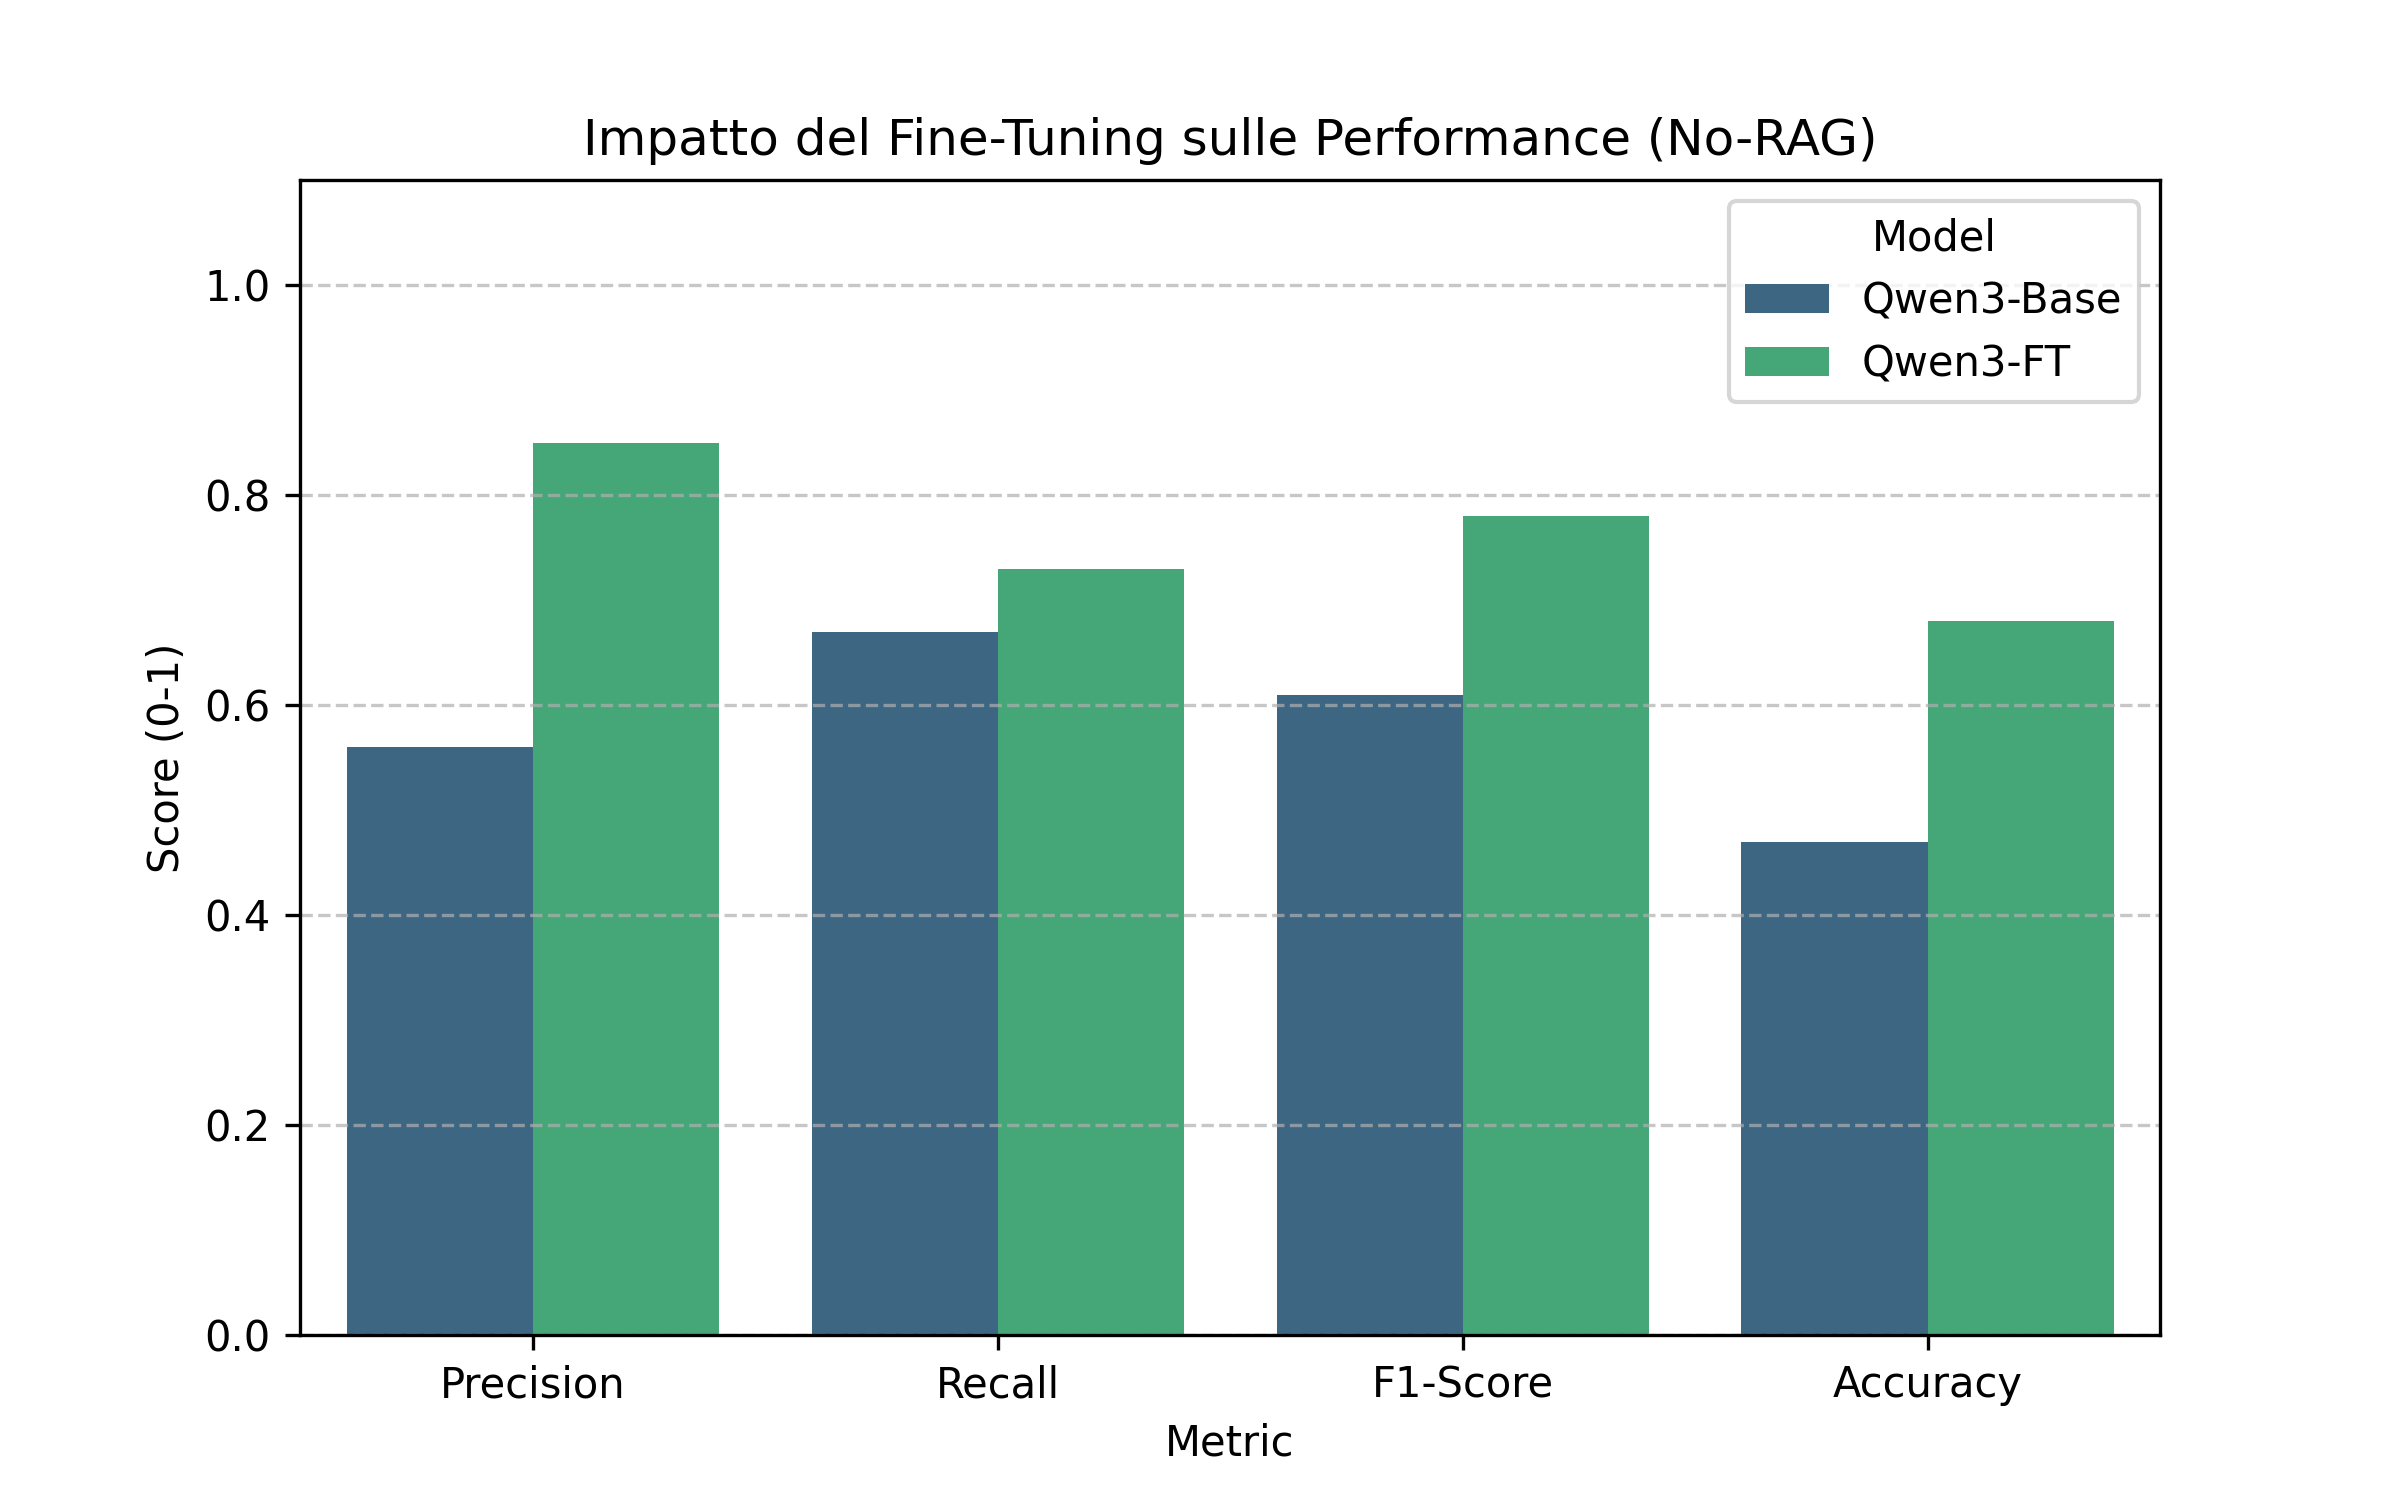
\includegraphics[width=0.9\textwidth]{images/ft_impact_chart_Qwen3.png}
    \caption{Impatto del Fine-Tuning (Qwen3) sulle metriche di performance (Accuracy, Precision, Recall, F1).}
    \label{fig:ft_impact_metrics_qwen}
\end{figure}

\begin{figure}[h]
    \centering
    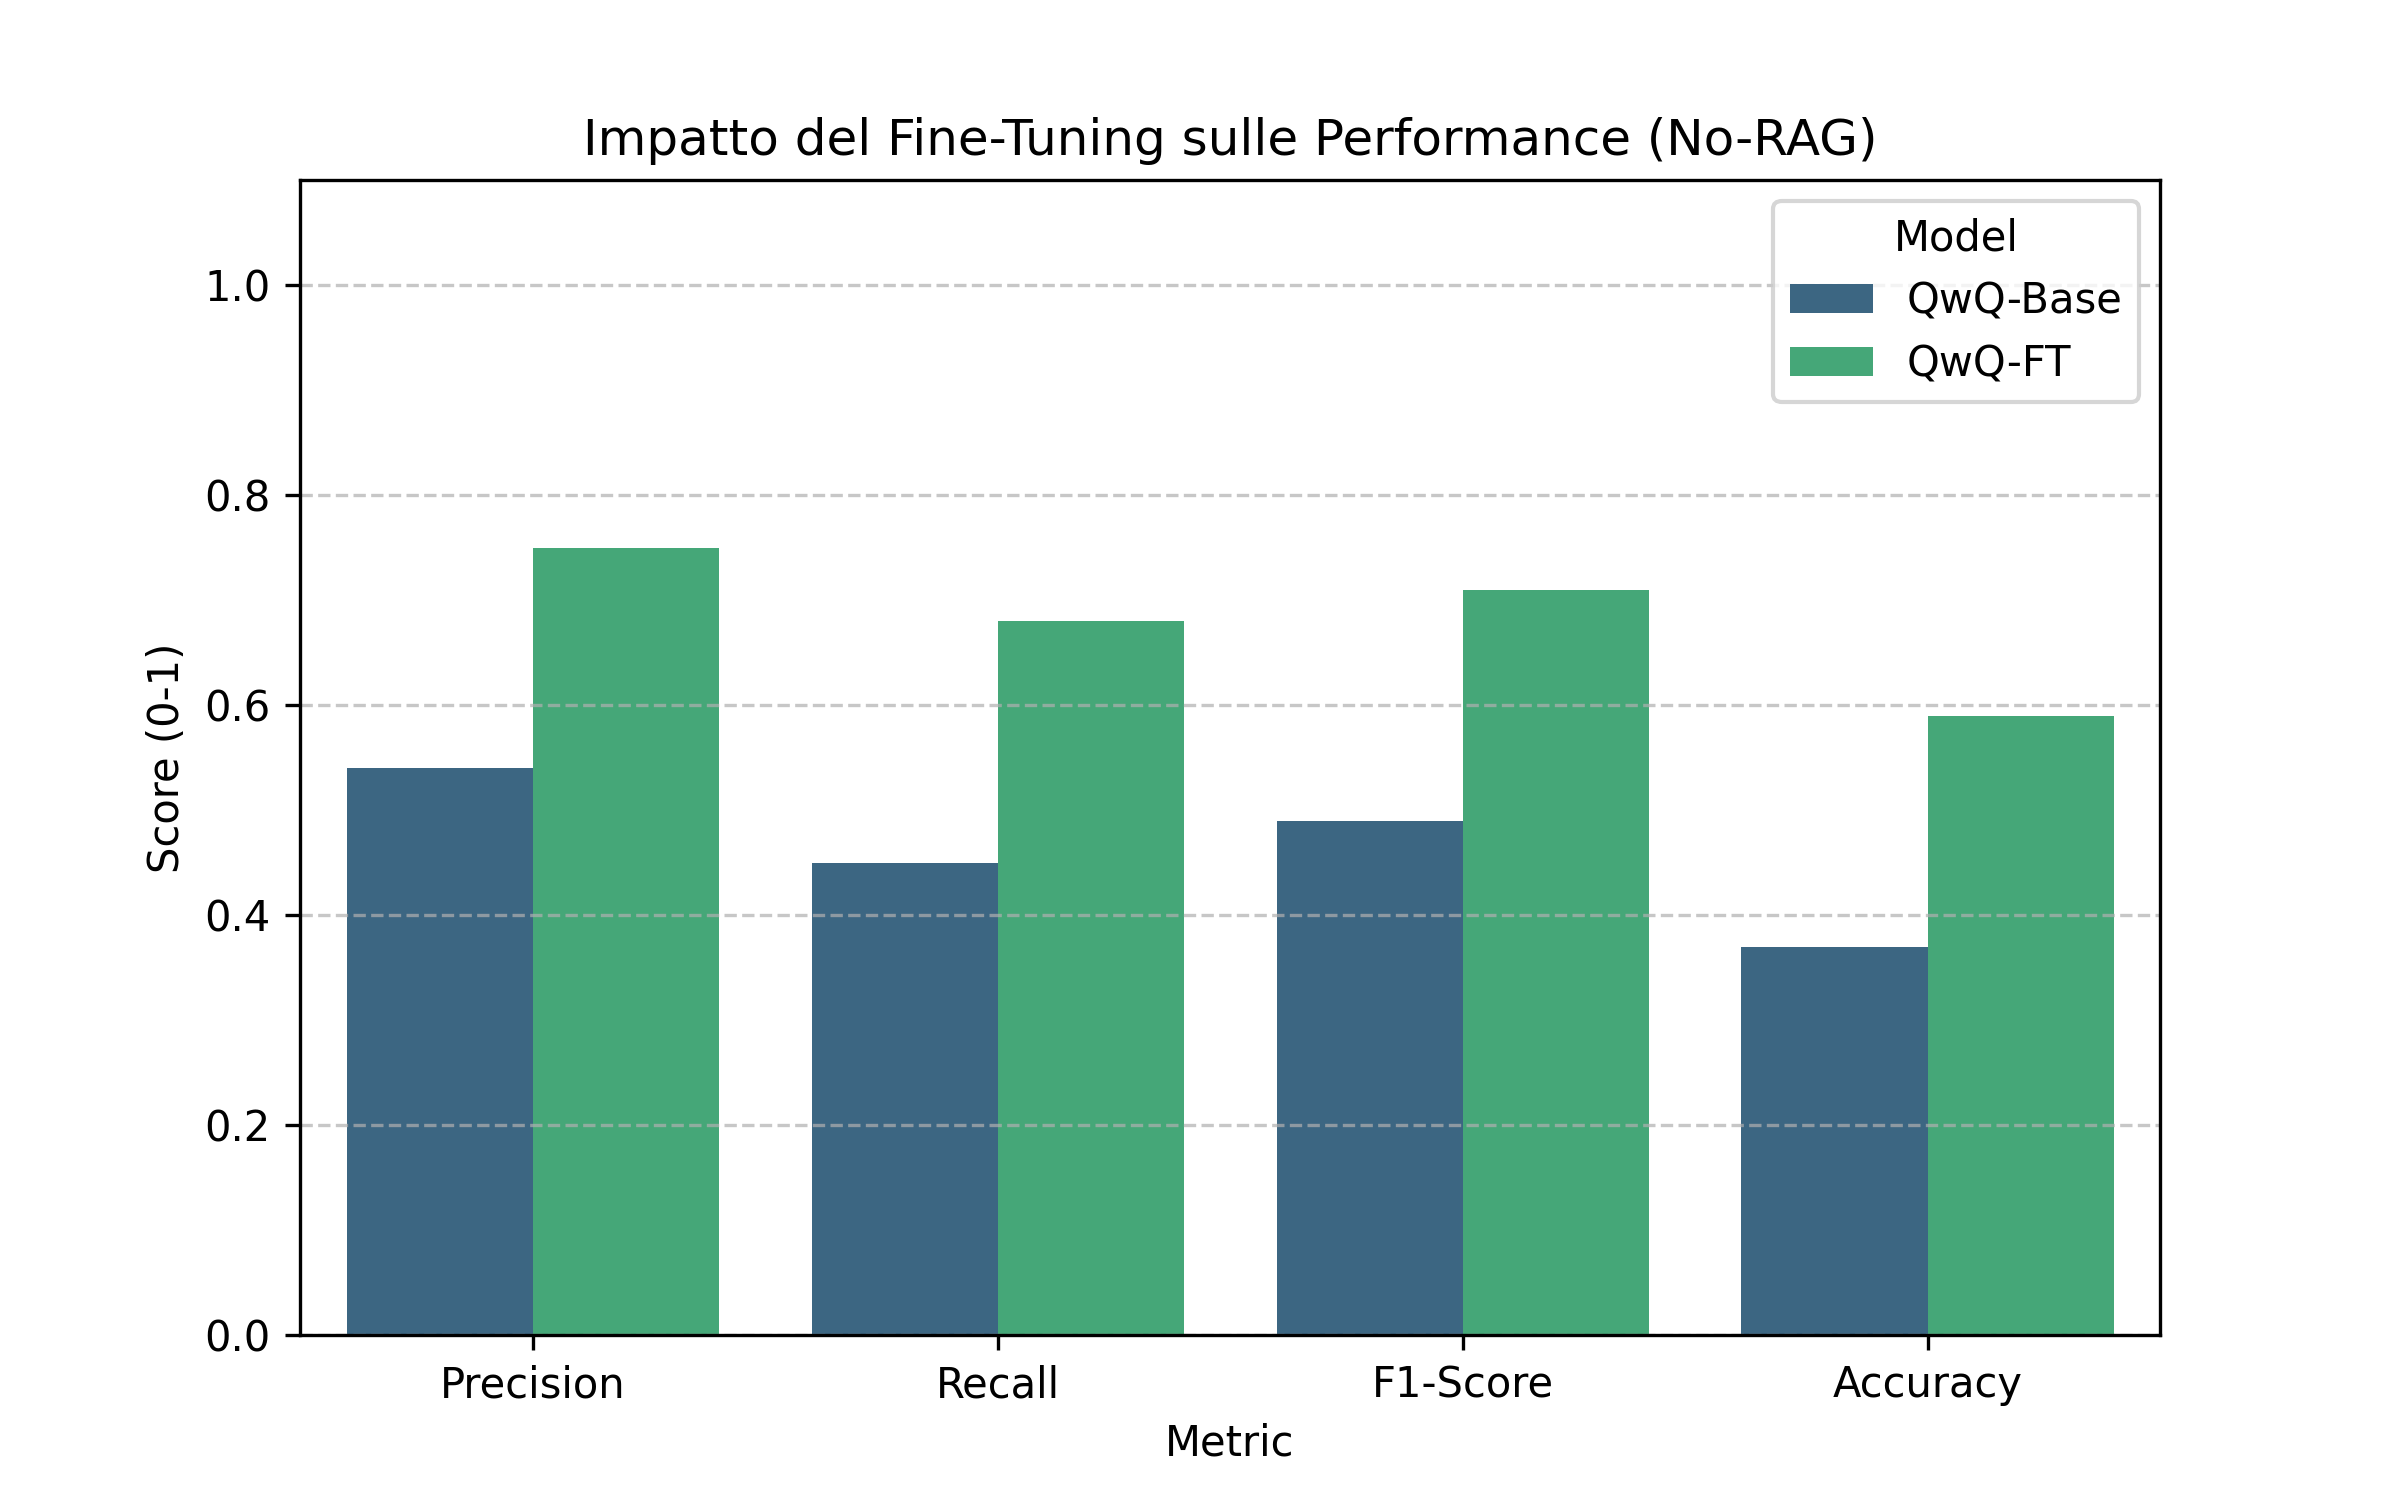
\includegraphics[width=0.9\textwidth]{images/ft_impact_chart_QwQ.png}
    \caption{Impatto del Fine-Tuning (QwQ) sulle metriche di performance (Accuracy, Precision, Recall, F1).}
    \label{fig:ft_impact_metrics_qwq}
\end{figure}

\newpage

Dall'analisi del grafico emergono trend distinti:
\begin{itemize}
    \item \textbf{Precision (Riduzione del Rumore):} È la metrica che ha beneficiato della trasformazione più radicale, smentendo l'ipotesi che il Fine-Tuning introduca overfitting. Al contrario, i dati mostrano che il modello Base soffriva di un elevato tasso di \textit{False Positives} (21 FP per Qwen3). Il modello FT ha imparato a discriminare i falsi allarmi, \textbf{abbattendo i FP a 5} e innalzando la Precision all'85\%.
    
    \item \textbf{Recall (Recupero della Conoscenza):} Per i modelli orientati al ragionamento (come QwQ), il Fine-Tuning è stato determinante per colmare il gap di conoscenza sintattica. Mentre il modello Base falliva nel riconoscere pattern specifici dell'AVM (con un alto tasso di FN), il processo di training ha permesso di "interiorizzare" le firme delle vulnerabilità, portando la Recall da un insufficiente 0.45 a un competitivo 0.675.
    
    \item \textbf{F1-Score e Affidabilità:} L'incremento dell'Accuracy non è solo numerico, ma qualitativo. Mentre l'accuratezza del modello Base era compromessa dall'incapacità di bilanciare sensibilità e specificità, il modello FT raggiunge un F1-Score di 0.78 (Qwen3), dimostrando di aver acquisito una comprensione operativa "utile": segnala le vulnerabilità quando ci sono e tace quando il codice è sicuro.
\end{itemize}

\begin{table}[h]
    \centering
    \caption{Dettaglio della Matrice di Confusione per i modelli testati (Test Set: 45 Contratti).}
    \label{tab:confusion_matrix_raw}
    \resizebox{\textwidth}{!}{%
    \begin{tabular}{l|cccc|c}
    \toprule
    \textbf{Modello} & \textbf{True Positive (TP)} & \textbf{True Negative (TN)} & \textbf{False Positive (FP)} & \textbf{False Negative (FN)} & \textbf{Totale} \\ \midrule
    Qwen3-32B (Base) & 27 & 4 & 21 & 13 & 65* \\
    \textbf{Qwen3-32B (FT)} & \textbf{29} & \textbf{5} & \textbf{5} & \textbf{11} & 50 \\ \midrule
    QwQ-32B (Base) & 18 & 4 & 15 & 22 & 59* \\
    \textbf{QwQ-32B (FT)} & \textbf{27} & \textbf{5} & \textbf{9} & \textbf{13} & 54 \\ \midrule
    
    \end{tabular}%
    }
    \vspace{0.2cm}
    \small
    \textit{*Nota: Per i modelli Base, la somma totale supera di molto 45 in quanto il modello tende a segnalare vulnerabilità multiple o errate (FP multipli) sullo stesso contratto.}
\end{table}

\subsection{Case Study Qualitativo}
\label{sec:case_study_rekey}

Per comprendere appieno il valore aggiunto del Fine-Tuning, è utile analizzare come i due modelli affrontano una vulnerabilità complessa basata su un'omissione: l'\textit{Unchecked Rekey To}.
In questo scenario, viene sottoposto ai modelli uno Smart Contract \textit{Stateless} (LogicSig) che approva un gruppo di due transazioni:
\begin{enumerate}
    \item \texttt{Gtxn[0]}: Una transazione di pagamento (Payment).
    \item \texttt{Gtxn[1]}: Un trasferimento di asset (AssetTransfer).
\end{enumerate}
Il codice è vulnerabile perché, mentre la seconda transazione controlla il campo \texttt{rekey\_to}, la prima (il pagamento) ne è priva, permettendo a un attaccante di prendere il controllo dell'account.

\subsubsection{Confronto delle Risposte}
Le Figure \ref{fig:resp_base} e \ref{fig:resp_ft} mostrano le risposte grezze generate rispettivamente dal modello Base e dal modello Fine-Tuned.
\newpage

\begin{figure}[h!]
    \centering
    \begin{tcolorbox}[colback=red!5!white, colframe=red!75!black, title=Risposta Modello Base (Qwen3-32B)]
    \small
    \textbf{<think>} 
    \[...\] Looking at the payment\_txn\_check for Gtxn[0], they check the type is Payment, amount is under 1M and close\_remainder\_to is zero. That seems good. \[...\]
    Now the asset\_transfer\_check for Gtxn[1]. They check rekey\_to is zero. \[...\]
    So all the relevant checks are present. No missing checks that would lead to the listed vulnerabilities. \\
    \textbf{</think>}
    
    \textbf{<final>} \\
    \textbf{Vulnerability: Not Vulnerable} \\
    Explanation: All relevant security checks are explicitly implemented for transaction fees, close\_remainder\_to, \textbf{rekey\_to}, asset\_close\_to, and receiver addresses.
    \textbf{</final>}
    \end{tcolorbox}
    \caption{Il Modello Base analizza i controlli presenti ma fallisce nel notare l'assenza del controllo sul Rekeying nella prima transazione, generando un Falso Negativo.}
    \label{fig:resp_base}
\end{figure}

\newpage

\begin{figure}[h!]
    \centering
    \begin{tcolorbox}[colback=green!5!white, colframe=green!75!black, title=Risposta Modello Fine-Tuned (Qwen3-32B-FT)]
    \small
    \textbf{<think>} \\
     \[...\]
    \textbf{Payment Transaction (Gtxn[0]):} \\
    - Type check: TxnType.Payment \\
    - Fee limit: `<= 1000` \checkmark\\
    - \textbf{Missing check: No validation of rekey\_to() field} 

    \[...\]
    
    \textbf{Asset Transfer Transaction (Gtxn[1]):} \\
    - Rekey to: == Global.zero\_address() \checkmark

     \[...\]
    
    The critical issue I notice is in the payment transaction validation. While the asset transfer transaction properly checks rekey\_to, the payment transaction completely omits this check. \\
    \textbf{</think>}
    
    \textbf{<final>} \\
    \textbf{Vulnerability: Unchecked Rekey To} \\
    Explanation: The payment transaction validation logic fails to check the rekey\_to field, allowing an attacker to include a rekey operation. \\
    \textbf{</final>}
    \end{tcolorbox}
    \caption{Il Modello FT adotta un approccio sistematico (checklist), identificando correttamente l'omissione nella prima transazione.}
    \label{fig:resp_ft}
\end{figure}
\newpage

\subsubsection{Discussione dell'Errore}
L'analisi comparativa evidenzia due comportamenti distinti:

\begin{itemize}
    \item \textbf{Generalizzazione Fallace del Modello Base:} Nel suo processo di pensiero (Figura \ref{fig:resp_base}), il modello nota che il \texttt{rekey\_to} è controllato nella seconda transazione. Tuttavia, nel verdetto finale, estende erroneamente questa proprietà all'intero contratto, dichiarando \textit{"All relevant security checks are explicitly implemented for... rekey\_to"}. Questa è una classica allucinazione da generalizzazione: il modello confonde la presenza \textit{locale} di un controllo con la sicurezza \textit{globale}.
    
    \item \textbf{Verifica Puntuale del Modello FT:} Il modello Fine-Tuned (Figura \ref{fig:resp_ft}) struttura il ragionamento separando nettamente le due transazioni (\texttt{Gtxn[0]} vs \texttt{Gtxn[1]}). Grazie all'addestramento su esempi di audit strutturati, il modello ha imparato a cercare attivamente l'assenza di vincoli, rilevando che la mancanza della riga \texttt{RekeyTo == ZeroAddress} nel blocco di pagamento costituisce una vulnerabilità critica.
\end{itemize}

Questo esempio dimostra come il Fine-Tuning non si limiti ad aggiungere conoscenza sintattica, ma modifichi il pattern di attenzione del modello, spostandolo da una lettura "riassuntiva" a una verifica "analitica" riga per riga.

\newpage

\subsection{Benchmark contro modelli SOTA}
\label{sec:benchmark_deepseek}

Per validare la reale efficacia del Fine-Tuning, i risultati ottenuti dai modelli specializzati (in particolare \texttt{Qwen3-32B-FT}) sono stati confrontati con \texttt{DeepSeek V3.2}, un modello allo Stato dell'Arte (SOTA) di dimensioni massicce, interrogato via API.

La Tabella mostra il confronto diretto tra il miglior modello Fine-Tuned e il modello SOTA.

\begin{table}[ht]
\centering
\resizebox{\textwidth}{!}{%
\begin{tabular}{l|cccc|cc}
\toprule
\textbf{Modello} & \textbf{Precision} & \textbf{Recall} & \textbf{F1-Score} & \textbf{Accuracy} & \textbf{FP} & \textbf{FN} \\ \midrule
\textbf{Qwen3-32B (FT)} & \textbf{0.85} & 0.725 & \textbf{0.784} & \textbf{0.680} & \textbf{5} & 11 \\ 
DeepSeek V3.2 (API) & 0.717 & \textbf{0.825} & 0.767 & 0.649 & 13 & \textbf{7} \\ \bottomrule
\end{tabular}%
}
\label{tab:rere}
\caption{Confronto tra il modello Fine-Tuned (Specialist) e DeepSeek V3.2 (Generalist).}
\end{table}

\begin{figure}[h]
    \centering
    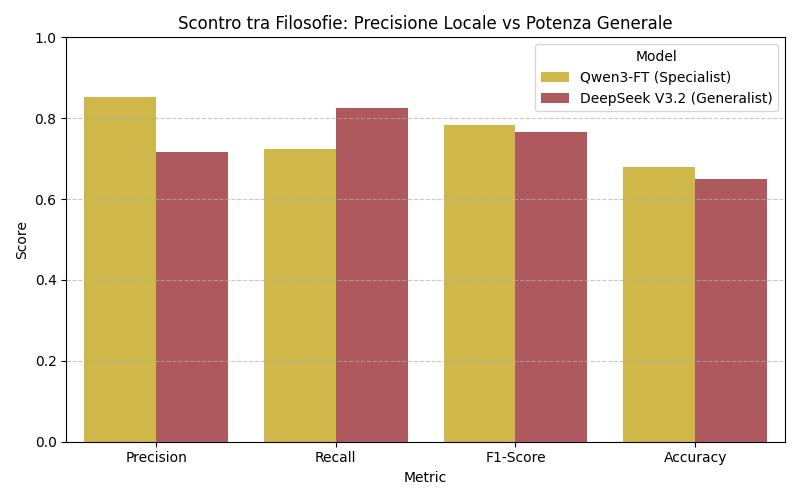
\includegraphics[width=0.9\textwidth]{images/ft_vs_deepseek.png}
    \caption{Confronto tra il modello Fine-Tuned (Specialist) e DeepSeek V3.2 (Generalist).}
    \label{fig:ft_vs_deepseek}
\end{figure}

Dall'analisi dei dati emerge una dinamica chiara che contrappone la "potenza bruta" alla "specializzazione":

\begin{itemize}
    \item \textbf{DeepSeek:} Grazie alla sua vasta conoscenza parametrica e capacità di ragionamento, DeepSeek ha ottenuto la \textbf{Recall più alta (0.825)}, identificando 33 vulnerabilità su 40 (solo 7 FN). Il modello riesce a trovare bug complessi che sfuggono al modello 32B, dimostrando che la capacità di ragionamento puro può compensare parzialmente la mancanza di training specifico.
    
    \item \textbf{Qwen3-FT:} Il modello Fine-Tuned, pur avendo una Recall inferiore (0.725), eccelle nella precisione. Con una \textbf{Precision dell'85\%} e solo \textbf{5 False Positives} (contro i 13 di DeepSeek), il modello specializzato si rivela molto più affidabile.
    
    \item \textbf{Accuracy e Affidabilità Globale:} Analizzando l'Accuracy, il modello FT supera il modello SOTA (\textbf{0.680 vs 0.649}). Questo dato, sebbene spesso meno informativo in dataset sbilanciati, qui conferma una tesi importante: DeepSeek "guadagna" Recall sparando nel mucchio (generando molti FP), mentre Qwen3-FT commette meno errori totali (somma di FP e FN).
    
    \item \textbf{F1-Score:} La sintesi finale premia l'equilibrio del modello specializzato (\textbf{0.784 vs 0.767}). Dimostra che un modello compatto (32B), se correttamente addestrato, può competere e superare un modello SOTA di ordine di grandezza superiore.
\end{itemize}

\section{Analisi Comparativa dell'Impatto del RAG}
\label{sec:rag_impact_analysis}

L'introduzione della pipeline RAG (Retrieval-Augmented Generation) rappresenta l'ultimo stadio di ottimizzazione del framework. In questa sezione analizziamo come l'iniezione di contesto dinamico influenzi le performance di tutte e cinque le configurazioni di modello testate, confrontando le metriche \textit{No-RAG} contro \textit{With-RAG}.

La Tabella \ref{tab:rag_comparison_full} riassume i delta prestazionali per tutte le metriche chiave.

\begin{table}[ht]
\centering
\resizebox{\textwidth}{!}{%
\begin{tabular}{l|cc|cc|cc}
\toprule
\textbf{Modello} & \multicolumn{2}{c|}{\textbf{Precision}} & \multicolumn{2}{c|}{\textbf{Recall}} & \multicolumn{2}{c}{\textbf{F1-Score}} \\ 
 & No-RAG & \textbf{With RAG} & No-RAG & \textbf{With RAG} & No-RAG & \textbf{With RAG} \\ \midrule
\textit{Base Models} & & & & & & \\
QwQ-32B & 0.57 & \textbf{0.83 (+0.26)} & 0.45 & \textbf{0.60 (+0.15)} & 0.51 & \textbf{0.70 (+0.19)} \\
Qwen3-32B & 0.56 & \textbf{0.90 (+0.34)} & 0.67 & 0.65 (-0.02) & 0.61 & \textbf{0.75 (+0.14)} \\ \midrule
\textit{Fine-Tuned Models} & & & & & & \\
\textbf{QwQ-32B (FT)} & 0.83 & \textbf{0.92 (+0.09)} & 0.72 & \textbf{0.87 (+0.15)} & 0.77 & \textbf{0.90 (+0.13)} \\
Qwen3-32B (FT) & 0.85 & \textbf{0.94 (+0.09)} & 0.72 & \textbf{0.82 (+0.10)} & 0.78 & \textbf{0.88 (+0.10)} \\ \midrule
\textit{SOTA} & & & & & & \\
DeepSeek V3.2 & 0.73 & \textbf{0.91 (+0.18)} & 0.82 & \textbf{0.97 (+0.15)} & 0.77 & \textbf{0.94 (+0.17)} \\ \bottomrule
\end{tabular}%
}
\caption{Impatto del RAG su Precision, Recall e F1-Score. I valori tra parentesi indicano il guadagno netto ($\Delta$) rispetto alla versione senza RAG.}
\label{tab:rag_comparison_full}
\end{table}

\newpage

\begin{figure}[h!]
    \centering
    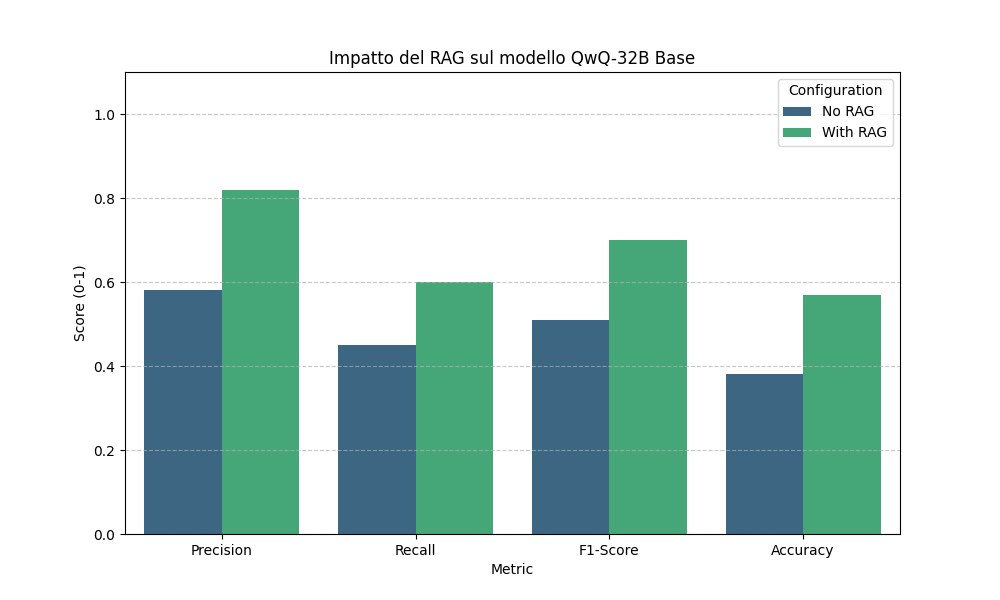
\includegraphics[width=\textwidth]{images/rag_impact_chart_qwq_base.png} 
    \caption{Confronto performance del modello QwQ-32B Base, con e senza RAG}
    \label{fig:rag_qwq_base}
\end{figure}

\begin{figure}[h!]
    \centering
    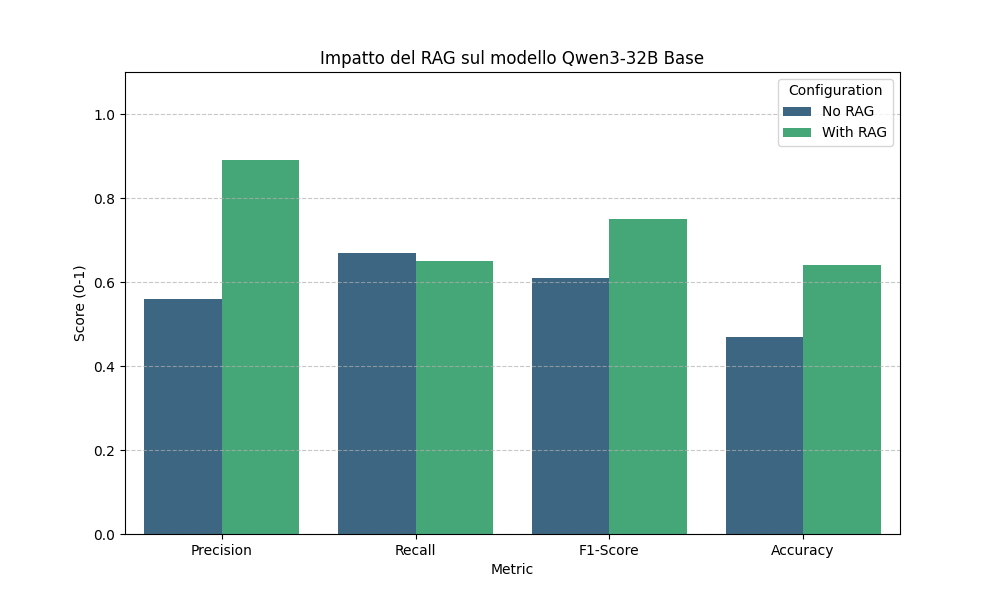
\includegraphics[width=\textwidth]{images/rag_impact_chart_qwen_base.png} 
    \caption{Confronto performance del modello Qwen3-32B Base, con e senza RAG}
    \label{fig:rag_qwen_base}
\end{figure}


\begin{figure}[h!]
    \centering
    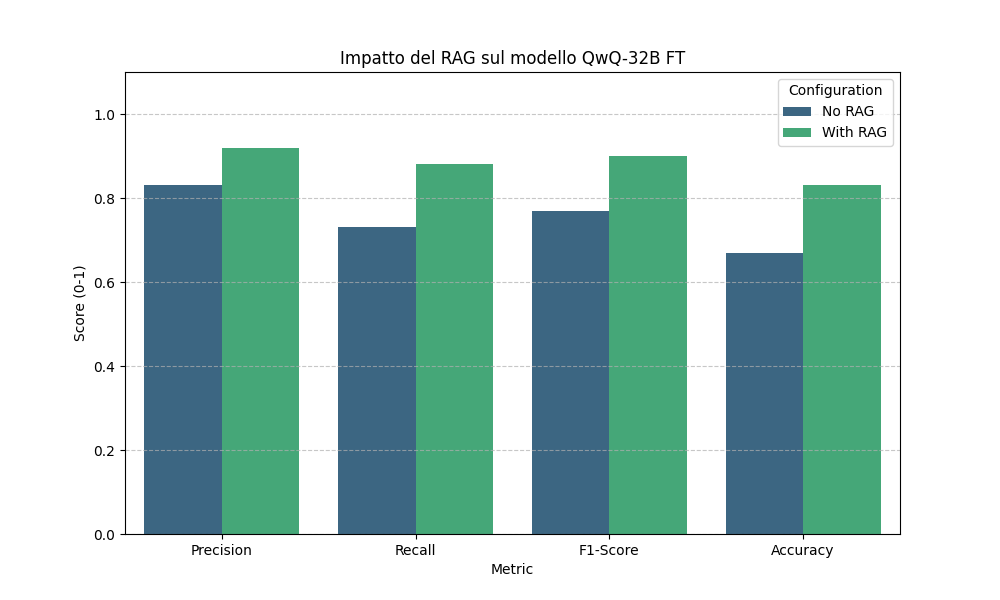
\includegraphics[width=\textwidth]{images/rag_impact_chart_qwq_ft.png} 
    \caption{Confronto performance del modello QwQ-32B FT, con e senza RAG}
    \label{fig:rag_qwq_ft}
\end{figure}

\begin{figure}[h!]
    \centering
    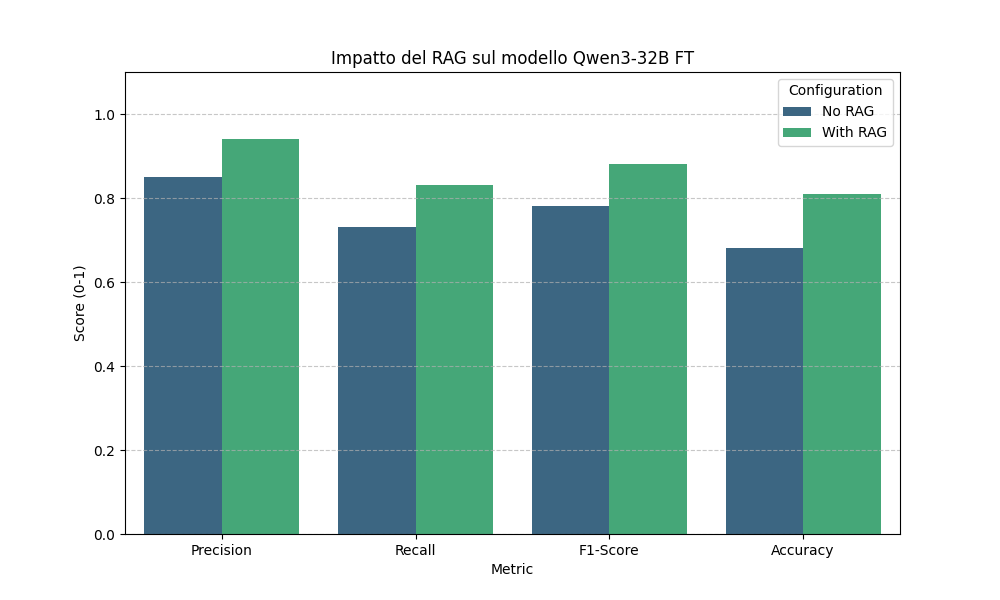
\includegraphics[width=\textwidth]{images/rag_impact_chart_qwen_ft.png} 
    \caption{Confronto performance del modello Qwen3-32B FT, con e senza RAG}
    \label{fig:rag_qwen_ft}
\end{figure}

\begin{figure}[h!]
    \centering
    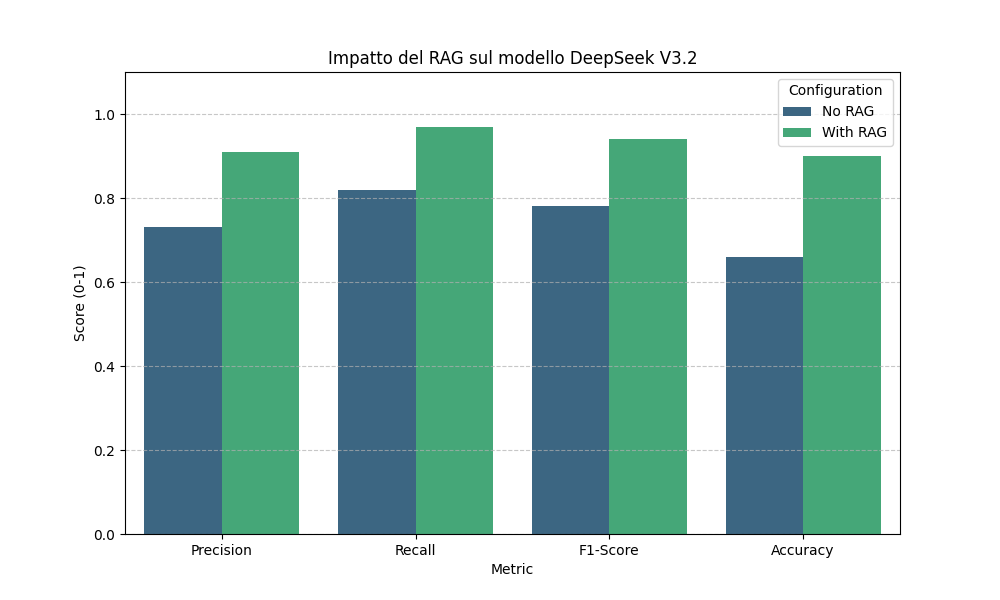
\includegraphics[width=\textwidth]{images/rag_impact_chart_deepseek.png} 
    \caption{Confronto performance del modello DeepSeek V3.2, con e senza RAG}
    \label{fig:rag_deepseek}
\end{figure}

\newpage

L'impatto del RAG si manifesta con dinamiche distinte in base alla maturità del modello sottostante.
Per i \textbf{Modelli Base} (QwQ/Qwen3), il retrieval agisce primariamente come "filtro di rumore": fornendo esempi reali, riduce drasticamente le allucinazioni (False Positives), portando la Precision dal 56\% all'89\% su Qwen3.
Nei \textbf{Modelli Fine-Tuned}, osserviamo la sinergia più efficace in termini di bilanciamento: il training pregresso garantisce la comprensione sintattica, mentre il RAG estende la memoria, permettendo al modello locale \texttt{QwQ-FT} di raggiungere un F1-Score di 0.90, rendendolo un'alternativa competitiva on-premise.
Infine, per il modello SOTA \textbf{DeepSeek V3.2}, il RAG colma le residue lacune di dominio: con una Recall del 97.5\% (un solo bug mancato su 40), dimostra che anche i modelli massivi necessitano di contesto specifico per saturare le performance su linguaggi di nicchia come PyTeal.

\subsection{Trade-off Computazionale e Latenza}
L'integrazione del RAG comporta inevitabilmente un costo computazionale aggiuntivo. Rispetto all'inferenza diretta, la pipeline ibrida introduce due fattori di overhead:
\begin{enumerate}
    \item \textbf{Latenza di Retrieval:} Il tempo necessario per l'embedding della query e la ricerca vettoriale (Vector Search) aggiunge circa 200-500ms per transazione analizzata.
    \item \textbf{Consumo di Token:} L'iniezione degli snippet di contesto nel prompt aumenta la finestra di input media del 40-60\%, incrementando proporzionalmente i tempi di pre-fill e i costi di inferenza (nel caso di API a pagamento).
\end{enumerate}
Tuttavia, considerando il dominio di applicazione (sicurezza degli Smart Contract), questo trade-off è ampiamente giustificato. In uno scenario di audit, dove l'accuratezza (F1-Score) è critica per prevenire perdite finanziarie, un incremento della latenza nell'ordine dei secondi è trascurabile rispetto al valore aggiunto della riduzione dei Falsi Negativi.

\subsection{Sintesi dei Risultati}
L'analisi comparata dimostra che:
\begin{enumerate}
    \item \textbf{Il RAG è sempre additivo:} Nessun modello ha peggiorato significativamente le performance globali con l'aggiunta del contesto.
    \item \textbf{FT + RAG > Base + RAG:} Il Fine-Tuning è un prerequisito essenziale per massimizzare l'efficacia del retrieval. QwQ-FT con RAG (F1 0.90) supera nettamente QwQ Base con RAG (F1 0.70), provando che il contesto non può sostituire completamente l'addestramento.
    \item \textbf{Gap SOTA ridotto:} La nostra soluzione locale (QwQ-FT + RAG) raggiunge un F1 di 0.90, distaccandosi di soli 4 punti percentuali dalla soluzione SOTA via API (0.94), validando la fattibilità di audit di sicurezza avanzati eseguiti on-premise.
\end{enumerate}

\chapter{Conclusioni e Sviluppi Futuri}
\section{Sintesi del Lavoro e Contributi Principali}
Questa tesi ha affrontato la sfida della rilevazione automatizzata di vulnerabilità negli Smart Contract Algorand (PyTeal), un ecosistema applicativo finora ampiamente trascurato dalla letteratura scientifica dominante. 
L'obiettivo primario è stato esplorare come superare le limitazioni dei Large Language Models generalisti, i quali, se applicati in modalità \textit{Zero-Shot}, tendono a generare output imprecisi e "allucinazioni".

Per risolvere questa criticità, abbiamo progettato una pipeline modulare e \textit{LLM-Centric} che valuta l'impatto di due approcci metodologici distinti: l'adattamento del dominio tramite \textbf{Fine-Tuning supervisionato} e l'iniezione di contesto dinamico tramite \textbf{Retrieval-Augmented Generation (RAG)}.

\section{Risultati Conseguiti}
I risultati sperimentali dimostrano chiaramente che l'impatto e la necessità di queste tecniche variano in modo significativo in funzione della scala e della maturità del modello linguistico adottato.

Per i modelli SOTA di grossa taglia (come DeepSeek V3.2) non necessitano di un addestramento specifico tramite Fine-Tuning. La loro vasta conoscenza parametrica e le elevate capacità di ragionamento nativo fanno sì che sia sufficiente affiancare il RAG per ottenere prestazioni eccellenti. Attraverso il solo \textit{In-Context Learning} basato sugli esempi recuperati dinamicamente, DeepSeek V3.2 ha raggiunto un F1-Score di 0.94 e una Recall quasi perfetta (97.5\%).

Al contrario, il \textbf{Fine-Tuning} è indispensabile in uno scenario ben specifico: l'utilizzo di modelli locali di taglia media (32B parametri) in ambienti \textit{on-premise}. Per questi modelli, il RAG da solo non è sufficiente a colmare le lacune di comprensione della sintassi PyTeal. Tuttavia, applicando il Fine-Tuning per infondere la conoscenza di base e combinandolo successivamente con il RAG, il modello locale \texttt{QwQ-32B} ha raggiunto un eccellente F1-Score di \textbf{0.90}. 

Dai risultati ottenuti possiamo rispondere alle seguenti domande di ricerca.

\subsection{Sull'utilità del Fine-Tuning} 
In linea di massima, i risultati dimostrano che l'addestramento specifico tramite Fine-Tuning non è strettamente necessario, se non in scenari applicativi molto ristretti. La sua utilità si concretizza esclusivamente quando si è vincolati all'uso di modelli locali di taglia media (es. 32B parametri) in ambienti privati (\textit{on-premise}), dove è indispensabile colmare una profonda lacuna sintattica di base del modello. Tuttavia, i dati evidenziano chiaramente che i modelli di grossa taglia (SOTA) ottengono risultati nettamente superiori sfruttando semplicemente l'\textit{In-Context Learning}. Possedendo già un'eccellente capacità di ragionamento nativa, per questi modelli massivi il dispendioso processo di Fine-Tuning risulta meno efficiente rispetto a un \textit{prompting} contestuale ben ingegnerizzato.

\subsection{Sull'utilità del RAG} 
Al contrario, il \textit{Retrieval-Augmented Generation} si conferma uno strumento assolutamente utile per una pipeline di audit. I modelli linguistici, per quanto grandi e potenti, tendono a ragionare in modo statistico e restano proni alle allucinazioni se interrogati in assenza di riferimenti concreti. Fornire informazioni di contesto mirate e dinamiche (come snippet di codice vulnerabile simile e descrizioni di sicurezza pertinenti) è il prerequisito fondamentale per far lavorare i modelli al massimo delle loro capacità.

\section{Limiti dello Studio}
Nonostante l'elevata accuratezza raggiunta, l'architettura proposta presenta alcune limitazioni strutturali e operative che è doveroso evidenziare.

In primo luogo, l'efficacia del modulo RAG è strettamente vincolata alla completezza e alla qualità del Database vettoriale. Di fronte a vulnerabilità \textit{zero-day} assolute o a pattern logici non mappati nella Knowledge Base, il sistema perde il beneficio dell'ancoraggio fattuale, dovendo fare affidamento unicamente sulla conoscenza parametrica del modello.

In secondo luogo, il sistema di Retrieval potrebbe soffrire di un bias semantico dovuto all'utilizzo esclusivo di descrizioni in linguaggio naturale. Se da un lato l'astrazione testuale (la \textit{Security Code Description}) \ref{sec:sec_code_desc} è cruciale per mitigare il rumore sintattico del codice grezzo, dall'altro introduce un potenziale punto di debolezza dovuto ad un'eventuale imprecisione, omissione o ambiguità dell'LLM durante la generazione del testo. Questo può deviare drasticamente la ricerca portando al recupero di contesto irrilevante o fuorviante.

Infine, l'analisi mostra limiti nell'individuazione di vulnerabilità complesse di tipo \textit{cross-contract}. Il sistema attuale analizza solamente il contesto locale del contratto; tracciare le interazioni di stato globale tra molteplici Smart Contract interdipendenti eccede le attuali capacità del framework.

\section{Sviluppi Futuri}
La naturale evoluzione del framework proposto risiede nel superamento dell'attuale architettura lineare in favore di un paradigma basato su agenti (\textit{Agentic Workflow}). Sebbene la pipeline RAG implementata si sia dimostrata altamente efficace, essa opera secondo un flusso di esecuzione statico e predeterminato.

Dotando l'LLM della capacità di utilizzare strumenti esterni (\textit{Tool}), il sistema potrebbe decidere dinamicamente e iterativamente quali risorse chiamare in base al codice in esame. Un agente di sicurezza così concepito potrebbe integrare:
\begin{itemize}
    \item \textbf{Strumenti di Analisi Statica:} Per delegare l'individuazione di errori comuni e strutturali a tool automatici, permettendo all'agente LLM di concentrare le proprie capacità di ragionamento esclusivamente sulla logica del contratto e sulle vulnerabilità più complesse.
    \item \textbf{Compilatori Nativi:} permettendo all'agente di interrogare il compilatore PyTeal/TEAL in \textit{real-time} per validare la sintassi delle sue ipotesi, ricevendo log di errore da analizzare e correggere autonomamente prima di emettere il verdetto finale.
    \item \textbf{La Pipeline RAG come Tool:} anziché subire passivamente il contesto fornito all'inizio, l'agente potrebbe decidere in autonomia quando interrogare il Database vettoriale, formulando query multiple e affinando la ricerca in base ai primi indizi riscontrati nel codice target.
\end{itemize}

Questa flessibilità operativa abiliterebbe l'esecuzione di audit profondamente più completi. Un agente dotato di memoria, capace di raccogliere informazioni eterogenee da più strumenti e di navigare tra i file di un intero progetto potrebbe tracciare il flusso di esecuzione e lo stato globale attraverso molteplici contratti interdipendenti.

Parallelamente all'evoluzione architetturale, un ulteriore margine di sviluppo risiede nell'ottimizzazione del sistema di Retrieval. Per mitigare il rischio di bias semantico derivante dall'uso esclusivo di descrizioni in linguaggio naturale, la ricerca vettoriale potrebbe essere arricchita integrando astrazioni strutturali del codice. Ispirandosi alle metodologie adottate da framework recenti come \textbf{Vul-RAG} e \textbf{PropertyGPT}, si potrebbe affiancare alla descrizione testuale una rappresentazione del codice generalizzata. Questo approccio prevede l'estrazione delle sole firme delle funzioni o degli \textit{statement} logici, rimuovendo intenzionalmente identificatori specifici e nomi di variabili per astrarre il pattern di vulnerabilità. L'utilizzo di una query ibrida, che combina la semantica del linguaggio naturale con la struttura astratta del codice, permetterebbe di recuperare esempi storici strutturalmente allineati, massimizzando la precisione dell'\textit{In-Context Learning}. 

\backmatter
\printbibliography[heading=bibintoc, title={Bibliografia}]

\end{document}
